\documentclass[fleqn,10pt]{olplainarticle}
\usepackage{lineno}
\usepackage{graphicx}
% Use option lineno for line numbers 

\title{Support Vector Regression}

\author[1]{Tanishk Deoghare}
\affil[1]{Department of Financial Engineering New York University Tandon School of Engineering}

\keywords{SVR, SVM, Rademacher}

\begin{abstract}
This document serves as a comprehensive introduction to Support Vector Regression (SVR) and provides insights into recent advancements in this dynamic field. Beginning with a fundamental exploration of regression in machine learning, we embark on the journey of using data to predict real-valued labels with precision. While Support Vector Machines (SVM) are traditionally associated with classification tasks, we shift our focus towards specialized generalization bounds tailored for regression problems. These bounds, applicable to both finite and infinite hypothesis sets, rely on tools such as Rademacher Complexity to assess hypothesis set complexity. Additionally, we introduce the concept of pseudo-dimension, an extension of VC-dimension, specifically designed for regression. The document also comprehensively covers various regression algorithms, including linear regression, kernel ridge regression, support-vector regression, Lasso, and their online variants. Each algorithm is rigorously examined, along with accompanying learning guarantees. This document caters to both newcomers in the field and researchers seeking an in-depth understanding of Support Vector Regression and its recent developments.
\end{abstract}

\begin{document}

\flushbottom
\maketitle
\thispagestyle{empty}

\section*{Introduction}

This document serves a dual purpose: first, to provide an accessible introduction to Support Vector Regression, particularly aimed at those new to this swiftly evolving field. Second, it aims to offer an overview of recent advancements in this domain. We delve into the essential concept of regression in machine learning. This involves using data to predict, as accurately as possible, the real-valued labels of given points or items. Regression is a fundamental task in machine learning, with a wide array of practical applications. While SVM primarily focuses on classification problems, we now shift our attention to generalization bounds tailored for regression tasks. These bounds apply to both finite and infinite hypothesis sets. We take help from tools like Rademacher Complexity to gauge the complexity of hypothesis sets in regression. Additionally, we introduce a specialized measure of complexity, known as pseudo-dimension, which extends the concept of VC-dimension to regression. Various regression algorithms are introduced and dissected, including linear regression, kernel ridge regression, support-vector regression, Lasso, and several online variants of these techniques. Throughout, we meticulously examine the properties of these algorithms, along with their corresponding learning guarantees.


\section*{Recap of SVM}
SVM is a machine learning algorithm that is primarily used for classification tasks. It is designed to find a hyperplane (a line in 2D, a plane in 3D, and a hyperplane in higher dimensions) that best separates different classes in the feature space. In SVM classification, the objective is to find the hyperplane that maximizes the margin between different classes while minimizing classification errors. The output of an SVM classifier is a class label (e.g., 0 or 1 in binary classification, or one of several labels in multi-class classification). It can utilize the kernel trick to map the data into a higher-dimensional space, potentially making the models more expressive and capable of capturing complex relationships. This can be achieved by tuning the hyper-parameters such as the kernel choice and the regularization parameter. It is commonly used in tasks like text classification, image classification, and other problems where data needs to be categorized into different classes. 

\section*{Intuition behind using SVR for regression}
There was a need for a similar robust technique like SVM in regression tasks. Traditional regression methods like linear regression might not handle complex relationships between features and target variables very well. The idea of using Support Vector Regression (SVR) stems from the success of Support Vector Machines (SVM) in classification tasks. The concept of SVR arose from the idea of using a loss function that considers not only the deviation of predictions from actual values but also introduces a margin of tolerance. This loss function is designed to find a hyperplane that fits the data well within a certain margin of error. SVR is an extension of SVM to regression problems. In SVR, the goal is to minimize the error between predicted values and actual values while allowing for a specified margin of tolerance (controlled by a hyperparameter). SVR identifies a subset of training examples (support vectors) that are critical in determining the hyperplane. These are the data points that are closest to the hyperplane or within the margin. Like SVM, SVR can also use the kernel trick to map the data into a higher-dimensional space, potentially capturing complex, non-linear relationships between features and the target variable. SVR allows for flexibility in modeling complex relationships while controlling over-fitting by adjusting the margin of tolerance. This balance is crucial in building accurate regression models. SVR's theoretical foundations are based on optimization theory, convex optimization, and the concept of reproducing kernel Hilbert spaces. These provide a solid mathematical framework for understanding and using SVR.

\section*{Methods and Materials}


\section{The Problem of Regression}
We first introduce the learning problem of regression. Let \(X\) denote the input space
and \(Y\) a measurable subset of \(\mathbb{R}\). Here, we will adopt the stochastic scenario and
will denote by \(D\) a distribution over \(X \times Y\). The deterministic scenario is a straightforward special case where input points admit a unique label determined by a target function \(f : X \to Y\).

In all supervised learning problems, the learner receives a labeled sample $S = \{(x_1, y_1), \ldots, (x_m, y_m)\}$ \( \in (X \times Y)^m \) drawn independently and identically according to $D$. Since the labels are real numbers, it is not reasonable to expect the learner to predict the exact label when it is unique or its average label. Instead, we aim for predictions to be close to the correct ones. This is the key distinction between regression and classification: in regression, the measure of error is based on the magnitude of the difference between the predicted real-valued label and the true or correct one, rather than on their equality or inequality. We denote by $L: Y \times Y \to \mathbb{R}^+$ the loss function used to measure the magnitude of error. The most common loss function in regression is the squared loss $L_2$ defined by $L(y; y_0) = |y_0 - y|^2$ for all $y, y_0 \in Y$, or, more generally, an $L_p$ loss defined by $L(y; y_0) = |y_0 - y|^p$, for some $p \geq 1$ and all $y, y_0 \in Y$.

Given a hypothesis set $H$ of functions mapping $X$ to $Y$, the regression problem involves using the labeled sample $S$ to find a hypothesis $h \in H$ with small expected loss or generalization error $R(h)$ with respect to the target function $f$:
\[R(h) = E_{(x,y) \sim D} \left[L\left(h(x), y\right)\right]\]

As in the previous chapters, the empirical loss or error of $h \in H$ is denoted by $\hat{R}_S(h)$ and defined by
\[\hat{R}_S(h) = \frac{1}{m} \sum_{i=1}^m L\left(h(x_i), y_i\right)\]

In the common case where $L$ is the squared loss, this represents the mean squared error of $h$ on the sample $S$.

When the loss function $L$ is bounded by some $M > 0$, that is $L(y_0; y) \leq M$ for all $y, y_0 \in Y$, or more strictly, $L(h(x); y) \leq M$ for all $h \in H$ and $(x, y) \in X \times Y$, the problem is referred to as a bounded regression problem. Many of the theoretical results presented in the following sections are based on this assumption. The analysis of unbounded regression problems is technically more complex and typically requires different types of assumptions.


\section{Generalization Bounds and Accuracy of Prediction}

A generalization bound is a mathematical inequality or formula that provides an upper limit on how much a machine learning model is expected to deviate from its performance on the training data to its performance on new, unseen data. In simpler terms, it gives us a theoretical guarantee of how well a model is likely to generalize to data it hasn't seen before. Generalization bounds are crucial in machine learning because the ultimate goal is to build models that can make accurate predictions or classifications on new, real-world data, not just on the data they were trained on. These bounds help us assess the reliability and performance of a machine-learning algorithm. There are various types of generalization bounds, and they can be derived using different mathematical techniques. Common types include:
\subsection{Rademacher Complexity Bounds:} These bounds are based on the concept of Rademacher random variables, which measure the ability of a hypothesis class (a set of possible models) to fit random labels on the data.
\subsection{VC-Dimension Bounds:} These bounds are based on the VC-dimension, which is a measure of the capacity or complexity of a hypothesis class. They provide insights into how well a class of functions can fit different labelings of the data.
\subsection{PAC (Probably Approximately Correct) Bounds:} These bounds come from the PAC learning framework, which focuses on algorithms that are probably (with high probability) close to correct. They provide guarantees on the expected error of a learned model.
\subsection{Margin Bounds:} These bounds are based on the concept of margin, which measures the confidence of a model's predictions. Models with larger margins tend to generalize better.
\subsection{Hoeffding Inequality and Concentration Inequalities:} These are probability inequalities that can be used to derive generalization bounds.
\\\\
These bounds are used to guide model selection, tune hyperparameters, and assess the suitability of a machine learning algorithm for a given problem. They provide a way to quantify and reason about the trade-off between model complexity, the size of the training set, and the expected performance on new data.

The following section presents learning guarantees for bounded regression problems. We start with the simple case of a finite hypothesis set.

\section{Finite hypothesis sets}

In the case of a finite hypothesis, we can derive a generalization bound for regression by a straightforward application of Hoeffding's inequality and the union bound.

\textbf{Theorem 1.1} Let $L$ be a bounded loss function. Assume that the hypothesis set $H$ is finite. Then, for any $\delta > 0$, with probability at least $1 - \delta$, the following inequality holds for all $h \in H$:
\[ R(h) \leq \hat{R}_S(h) + M \sqrt{\frac{\log |H| + \log \frac{1}{\delta}}{2m}} \]

\textbf{Proof:} By Hoeffding's inequality, since $L$ takes values in $[0, M]$, for any $h \in H$, the following holds:
\[ \mathbb{P}\left(R(h) - \hat{R}_S(h) > \epsilon\right) \leq e^{-2m\epsilon^2 / M^2} \]

Thus, by the union bound, we can write
\[ \mathbb{P}\left(\exists h \in H : R(h) - \hat{R}_S(h) > \epsilon\right) \leq |H|e^{-2m\epsilon^2 / M^2} \]

Setting the right-hand side to be equal to $\delta$ yields the statement of the theorem.

With the same assumptions and using the same proof, a two-sided bound can be derived: with probability at least $1 - \delta$, for all $h \in H$,
\[ |R(h) - \hat{R}_S(h)| \leq M \sqrt{\frac{\log |H| + \log \frac{2}{\delta}}{2m}} \]

These learning bounds are similar to those derived for classification. In fact, they coincide with the classification bounds given in the inconsistent case when $M = 1$. Thus, all the remarks made in that context apply identically here. In particular, a larger sample size $m$ guarantees better generalization; the bound increases as a function of $\log |H|$ and suggests selecting, for the same empirical error, a smaller hypothesis set. This is an instance of Occam's razor principle for regression. In the next sections, we present other instances of this principle for the general case of infinite hypothesis sets using the notions of Rademacher complexity and pseudodimension.

\subsection{Rademacher complexity bounds}

Here, we show how the Rademacher complexity bounds of theorem 3.3 can be used to derive generalization bounds for regression in the case of the family of $L_p$ loss functions. We first show an upper bound for the Rademacher complexity of a relevant family of functions.

\textbf{Proposition 11.2 (Rademacher complexity of $\boldsymbol{\mu}$-Lipschitz loss functions)} Let $L: Y \times Y \to \mathbb{R}$ be a non-negative loss upper bounded by $M > 0$ ($L(y; y_0) \leq M$ for all $y; y_0 \in Y$) and such that for any fixed $y_0 \in Y$, $y \mapsto L(y; y_0)$ is $\mu$-Lipschitz for some $\mu > 0$. Then, for any sample $S = ((x_1; y_1), \ldots, (x_m; y_m))$, the Rademacher complexity of the family $G = \{ (x, y) \mapsto L(h(x); y) : h \in H \}$ is upper bounded as follows:
\[ \hat{R}_S(G) \leq \mu \hat{R}_S(H) \]

\textbf{Proof:} Since for any fixed $y_i$, $y \mapsto L(y; y_i)$ is $\mu$-Lipschitz, by Talagrand's contraction lemma (lemma 5.7), we can write
\[
\hat{R}_S(G) = \frac{1}{m} \mathbb{E}_\sigma \left[ \sum_{i=1}^m \sigma_i L(h(x_i), y_i) \right] \leq \frac{1}{m} \mathbb{E}_\sigma \left[ \sum_{i=1}^m \sigma_i \mu h(x_i) \right] = \mu \hat{R}_S(H)
\]

which completes the proof.

\textbf{Theorem 11.3 (Rademacher complexity regression bounds)} Let $L: Y \times Y \to \mathbb{R}$ be a non-negative loss upper bounded by $M > 0$ ($L(y; y_0) \leq M$ for all $y; y_0 \in Y$) and such that for any fixed $y_0 \in Y$, $y \mapsto L(y; y_0)$ is $\mu$-Lipschitz for some $\mu > 0$. Then, for any $\delta > 0$, with probability at least $1 - \delta$, over a sample $S$ of size $m$, the following inequalities hold for all $h \in H$:
\[
\begin{aligned}
&\mathbb{E}_{(x,y) \sim D} \left[ L(x, y) \right] \leq \frac{1}{m} \sum_{i=1}^m L(x_i, y_i) + 2\mu R_m(H) + M\sqrt{\frac{2\log(1/\delta)}{m}} \\
&\mathbb{E}_{(x,y) \sim D} \left[ L(x, y) \right] \leq \frac{1}{m} \sum_{i=1}^m L(x_i, y_i) + 2\mu \hat{R}_S(H) + 3M\sqrt{\frac{2\log(2/\delta)}{m}}
\end{aligned}
\]

\textbf{Proof:} Since for any fixed $y_i$, $y \mapsto L(y, y_i)$ is $\mu$-Lipschitz, by Talagrand's contraction lemma (lemma 5.7), we can write
\[
RS(G) = \frac{1}{m} \mathbb{E}_\sigma \left[ \sum_{i=1}^m \sigma_i L(h(x_i), y_i) \right] \leq \frac{1}{m} \mathbb{E}_\sigma \left[ \sum_{i=1}^m \sigma_i \mu h(x_i) \right] = \mu \hat{R}_S(H).
\]

Combining this inequality with the general Rademacher complexity learning bound of theorem 3.3 completes the proof. 

Let \( p \geq 1 \) and assume that \( |h(x) - y| \leq M \) for all \( (x, y) \in X \times Y \) and \( h \in H \). Then, since for any \( y_0 \) the function \( y \mapsto |y - y_0|^p \) is \( pM^{p-1} \)-Lipschitz for \( (y - y_0) \in [-M, M] \), the theorem applies to any \( L_p \)-loss. As an example, for any \( \delta > 0 \), with probability at least \( 1 - \delta \) over a sample \( S \) of size \( m \), each of the following inequalities holds for all \( h \in H \):
\[
\mathbb{E}_{(x,y) \sim D} \left[ \left| h(x) - y \right|^p \right] \leq \frac{1}{m} \sum_{i=1}^m \left|  h(x_i) - y_i  \right|^p + 2pM^{p-1}R_m(H) + M^p \sqrt{\frac{\log\left(\frac{1}{\delta}\right)}{2m}}
\]

As in the case of classification, these generalization bounds suggest a trade-off between reducing the empirical error, which may require more complex hypothesis sets, and controlling the Rademacher complexity of \(H\), which may increase the empirical error. An important benefit of the last learning bound of the theorem is that it is data-dependent. This can lead to more accurate learning guarantees. The upper bounds on \(R_m(H)\) or \(R_S(H)\) for kernel-based hypotheses (theorem 6.12) can be used directly here to derive generalization bounds in terms of the trace of the kernel matrix or the maximum diagonal entry.


\subsection{Pseudodimension bounds}

As previously discussed in the case of classification, it is sometimes computationally hard to estimate the empirical Rademacher complexity of a hypothesis set. Hence, we introduce other measures of the complexity of a hypothesis set such as the VC-dimension, which are purely combinatorial and typically easier to compute or upper bound. However, the notion of shattering or that of VC-dimension introduced for binary classification is not readily applicable to real-valued hypothesis classes.

We first introduce a new notion of shattering for families of real-valued functions.

\textbf{Definition 11.4 (Shattering)} Let $G$ be a family of functions from a set $Z$ to $\mathbb{R}$. A set \(\{z_1, \ldots , z_m\} \subseteq X\) is said to be shattered by $G$ if there exist \(t_1, \ldots , t_m \in \mathbb{R} \) such that,
\[
\left| \left\{
\begin{array}{cccc}
\begin{bmatrix}
\mathrm{sgn}(g(z_1) - t_1) \\
\vdots \\
\mathrm{sgn}(g(z_m) - t_m)
\end{bmatrix} & : & g \in G
\end{array}
\right\} \right| = 2^m
\]


When they exist, the threshold values $t_1, \ldots , t_m$ are said to witness the shattering. Thus, \(\{z_1, \ldots , z_m\}\) is shattered if for some witnesses $t_1, \ldots , t_m$, the family of functions $G$ is rich enough to contain a function going above a subset $A$ of the set of points $I = \{(z_i, t_i) : i \in [m]\}$ and below the others ($I - A$), for any choice of the subset $A$. Figure 11.1 illustrates this shattering in a simple case. The notion of shattering naturally leads to the following definition.

\textbf{Definition 11.5 (Pseudodimension)} Let $G$ be a family of functions mapping from $X$ to $\mathbb{R}$. Then, the pseudo-dimension of $G$, denoted by $\text{Pdim}(G)$, is the size of the largest set shattered by $G$.

By definition of the shattering just introduced, the notion of pseudo-dimension of a family of real-valued functions $G$ coincides with that of the VC-dimension of the corresponding thresholded functions mapping $X$ to $\{0, 1\}$:
\[
Pdim(G) = VCdim\left(\{(x, t) \mapsto 1_{(g(x) - t > 0)}: g \in G\}\right)
\]


Figure 11.2 illustrates this interpretation. In view of this interpretation, the following two results follow directly the properties of the VC-dimension.

\textbf{Theorem 11.6} The pseudo-dimension of hyperplanes in $\mathbb{R}^N$ is given by
\[ \text{Pdim}\left(\{x \mapsto w \cdot x + b : w \in \mathbb{R}^N, b \in \mathbb{R}\}\right) = N + 1 \]

\textbf{Theorem 11.7} The pseudo-dimension of a vector space of real-valued functions $H$ is equal to the dimension of the vector space:
\[ \text{Pdim}(H) = \dim(H) \]

The following theorem gives a generalization bound for bounded regression in terms of the pseudo-dimension of a family of loss function $G = \{ z = (x, y) \mapsto L(h(x), y) : h \in H\}$ associated to a hypothesis set $H$. The key technique to derive these bounds consists of reducing the problem to that of classification by making use of the following general identity for the expectation of a random variable $X$:
\[ \mathbb{E}[X] = -\int_{-\infty}^{0} \mathbb{P}[X < t]dt + \int_0^{\infty} \mathbb{P}[X > t]dt \]

which holds by definition of the Lebesgue integral. In particular, for any distribution $D$ and any non-negative measurable function $f$, we can write
\[ \mathbb{E}_{z \sim D}[f(z)] = \int_0^{\infty} P_{z \sim D}[f(z) > t]dt \]

\textbf{Theorem 11.8} Let $H$ be a family of real-valued functions and $G = \{(x, y) \mapsto L(h(x), y) : h \in H\}$ the family of loss functions associated to $H$. Assume that $\text{Pdim}(G) = d$ and that the loss function $L$ is non-negative and bounded by $M$. Then, for any $\delta > 0$, with probability at least $1 - \delta$ over the choice of an i.i.d. sample $S$ of size $m$ drawn from $D^m$, the following inequality holds for all $h \in H$:
\[ R(h) \leq \hat{R}_S(h) + M\sqrt{\frac{2d \log \frac{e m}{d}}{m}} + M\sqrt{\frac{\log (1/\delta)}{2m}} \]

\textbf{Proof:} Let \(S\) be a sample of size \(m\) drawn i.i.d. according to \(D\) and let \(\hat{D}\) denote the empirical distribution defined by \(S\). For any \(h \in H\) and \(t \geq 0\), we denote by \(c(h, t)\) the classifier defined by \(c(h, t):(x, y) \mapsto 1_{L(h(x),y) > t}\). The error of \(c(h, t)\) can be defined by
\[
R(c(h, t)) = \mathbb{P}_{(x,y) \sim D} [c(h, t)(x, y) = 1] = \mathbb{P}_{(x,y) \sim D} [L(h(x), y) > t]
\]
Now, given the identity (11.5) and the fact that the loss function L is bounded by M, we can write:
\[
\left| R(h) - \widehat{R}_S(h) \right| =
\left| \mathbb{E}_{(x,y) \sim D} \left[ L(h(x), y) \right] - \mathbb{E}_{(x,y) \sim \widehat{D}} \left[ L(h(x), y) \right] \right|
\]
\[
= \int_{0}^{M} \left( \mathbb{P}_{( (x,y) \sim D} [L(h(x), y) > t] - \mathbb{P}_{( (x,y) \sim \widehat{D}} [L(h(x), y) > t] \right) \, dt
\]
\[
\leq M \sup_{t \in [0,M]} \left| \mathbb{P}_{( (x,y) \sim D} [L(h(x), y) > t]  - \mathbb{P}_{( (x,y) \sim \widehat{D}} [L(h(x), y) > t]  \right|
\]
\[
= M \sup_{t \in [0,M]} \left| R(c(h, t)) - \widehat{R}_S (c(h, t)) \right|
\]
This implies the following inequality:
\[
\mathbb{P} \left[ \sup_{h \in H} \left| R(h) - \widehat{R}_S(h) \right| > \epsilon \right]
\leq \mathbb{P} \left[ \sup_{h \in H \ t \in [0,M]} \left| R(c(h, t)) - \widehat{R}_S(c(h, t)) \right| > \frac{\epsilon}{M} \right]
\]


The right-hand side can be bounded using a standard generalization bound for classification (corollary 3.19) in terms of the VC-dimension of the family of hypotheses $\{c(h, t) : h \in H, t \in [0, M]\}$, which, by definition of the pseudo-dimension, is precisely $\text{Pdim}(G) = d$. The resulting bound coincides with (11.6). The notion of pseudo-dimension is suited to the analysis of regression as demonstrated by the previous theorem; however, it is not a scale-sensitive notion. There exists an alternative complexity measure, the fat-shattering dimension, that is scale sensitive and that can be viewed as a natural extension of the pseudo-dimension. Its definition is based on the notion of $\gamma$ shattering.

\textbf{Definition 11.9 ($\gamma$-shattering)}
Let \(G\) be a family of functions from \(\mathbb{Z}\) to \(\mathbb{R}\) and let \(\gamma > 0\).
A set \(\{z_1, \ldots, z_m\} \subseteq X\) is said to be \(\gamma\)-shattered by \(G\) if there exist \(t_1, \ldots, t_m \in \mathbb{R}\) such that for all \(y \in \{-1, +1\}^m\), there exists \(g \in G\) such that:
\[
\forall i \in [m], \quad y_i(g(z_i) - t_i) \geq \gamma.
\]
Thus, \(\{z_1, \ldots, z_m\}\) is \(\gamma\)-shattered if for some witnesses \(t_1, \ldots, t_m\), the family of functions \(G\) is rich enough to contain a function going at least \(\gamma\) above a subset \(A\) of the set of points \(I = \{(z_i, t_i) : i \in [m]\}\) and at least \(\gamma\) below the others \((I - A)\), for any choice of the subset \(A\).

\textbf{Definition 11.10 ($\gamma$-fat-dimension)}
The \(\gamma\)-fat-dimension of \(G\), \(\text{fat}_{\gamma}(G)\), is the size of the largest set that is \(\gamma\)-shattered by \(G\).

Finer generalization bounds than those based on the pseudo-dimension can be derived in terms of the \(\gamma\)-fat-dimension. However, the resulting learning bounds are not more informative than those based on the Rademacher complexity, which is also a scale-sensitive complexity measure. Thus, we will not detail an analysis based on the \(\gamma\)-fat-dimension.


\textbf{Summarizing guarantees on hypothesis sets:}
\\The results of the previous sections show that, for the same empirical error, hypothesis sets with smaller complexity measured in terms of the Rademacher complexity or in terms of pseudo-dimension benefit from better generalization guarantees. One family of functions with relatively small complexity is that of linear hypotheses. In the subsequent section, we describe and analyze several algorithms based on that hypothesis set: linear regression, kernel ridge regression (KRR), support vector regression (SVR), and Lasso. These algorithms, in particular the last three, are extensively used in practice and often lead to state-of-the-art performance results.


\section{Formulating the regression problem}

Suppose we are given training data $\{(x_1, y_1), \ldots, (x_n, y_n)\} \subset X \times \mathbb{R}$, where $X$ denotes the space of input patterns (e.g., $X = \mathbb{R}^d$). These might be, for instance, exchange rates for some currency measured at subsequent days together with corresponding econometric indicators. In $\epsilon$-SV regression (Vapnik 1995), our goal is to find a function $f(x)$ that has at most $\epsilon$ deviation from the actually obtained targets $y_i$ for all the training data, and at the same time is as flat as possible. In other words, we do not care about errors as long as they are less than $\epsilon$, but will not accept any deviation larger than this. This may be important if you want to be sure not to lose more than $\epsilon$ money when dealing with exchange rates, for instance.

For pedagogical reasons, we begin by describing the case of linear functions $f$, taking the form

\[f(x) = \langle w, x \rangle + b\]


with $w \in X$ and $b \in \mathbb{R}$, where $\langle \cdot, \cdot \rangle$ denotes the dot product in $X$. Flatness in the case of $(1)$ means that one seeks a small $w$. One way to ensure this is to minimize the norm, i.e., $\|w\|^2 = \langle w, w \rangle$. We can write this problem as a convex optimization problem:
\[
\begin{aligned}
    \text{minimize} \quad & \frac{1}{2} \|w\|^2  \\
    \text{subject to} \quad
    \begin{cases}
    y_i - \langle w, x_i \rangle - b \leq \epsilon \\
    \langle w, x_i \rangle + b - y_i \leq \epsilon
    \end{cases}
\end{aligned}
\]

The tacit assumption in $(2)$ was that such a function $f$ actually exists that approximates all pairs $(x_i, y_i)$ with $\epsilon$ precision, or in other words, that the convex optimization problem is feasible. Sometimes, however, this may not be the case, or we may also want to allow for some errors. Analogously to the "soft margin" loss function (Bennett and Mangasarian 1992) which was used in SV machines by Cortes and Vapnik (1995), one can introduce slack variables $\xi_i, \xi_i^*$ to cope with otherwise infeasible constraints of the optimization problem $(2)$. Hence we arrive at the formulation stated in Vapnik (1995).

\[
\begin{aligned}
    \text{minimize} \quad & \frac{1}{2} \|w\|^2 + C \sum_{i=1}^n (\xi_i + \xi_i^*) \\
    \text{subject to} \quad 
    \begin{cases}
    y_i - \langle w, x_i \rangle - b \leq \epsilon + \xi_i \\
    \langle w, x_i \rangle + b - y_i \leq \epsilon + \xi_i^* \\
    \xi_i, \xi_i^* \geq 0
    \end{cases}
\end{aligned}
\]

The constant $C > 0$ determines the trade-off between the flatness of $f$ and the amount up to which deviations larger than $\epsilon$ are tolerated. This corresponds to dealing with a so-called $\epsilon$-insensitive loss function $|\xi|_\epsilon$ described by

\[
|\xi|_\epsilon =
\begin{cases}
    0 & \text{if } |\xi| \leq \epsilon \\
    |\xi| - \epsilon & \text{otherwise}
\end{cases}
\]

\begin{figure}
    \centering
    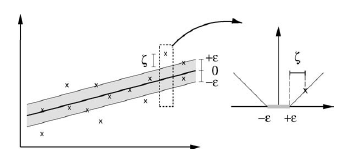
\includegraphics[width=0.8\linewidth]{Figure 1.png}
    \caption{The soft margin loss setting for a linear SVM (from Schölkopf and Smola, 2002}
    \label{fig:your_label}
\end{figure}

Figure 1 depicts the situation graphically. Only the points outside the shaded region contribute to the cost, as the deviations are penalized linearly. It turns out that in most cases the optimization problem $(3)$ can be solved more easily in its dual formulation. Moreover, as we will see in subsequent sections, the dual formulation provides the key for extending SV machine to nonlinear functions. Hence we will use a standard dualization method utilizing Lagrange multipliers, as described in e.g. Fletcher (1989).

\subsection{Support Vector Regression (SVR)}

SVR attempts to fit a "tube" with width $\varepsilon$ to the data. Training data within the $\varepsilon$ tube (blue points) incur no loss. It is inspired by the SVM algorithm presented for classification in Chapter 5. The main idea of the algorithm consists of fitting a tube of width $\varepsilon > 0$ to the data, as illustrated by Figure 11.4. Similar to binary classification, this defines two sets of points: those falling inside the tube, which are $\varepsilon$-close to the predicted function and thus not penalized, and those falling outside, which are penalized based on their distance to the predicted function, similar to the penalization used by SVMs in classification.

\begin{figure}
    \centering
    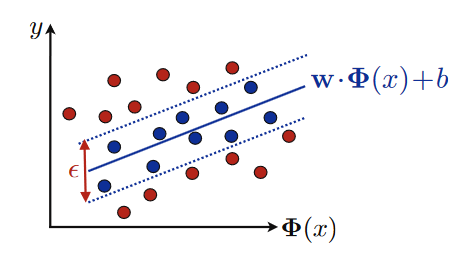
\includegraphics[width=0.8\linewidth]{SVR regression coloured.png}
    \caption{For N = 1, linear regression consists of finding the line of best fit, measured in terms of the squared loss.}
    \label{fig:your_label}
\end{figure}


The hypothesis set $H$ consists of linear functions: $H = \{x \mapsto w \cdot \varphi(x) + b: w \in \mathbb{R}^N, b \in \mathbb{R}\}$, where $\varphi$ is the feature mapping corresponding to some Positive Definite Semi-Definite (PDS) kernel $K$. The optimization problem for SVR can be written as follows:

\begin{align}
\min_{w, b} \frac{1}{2}\|w\|^2 + C \sum_{i=1}^m \left|y_i - \left(w \cdot \varphi(x_i) + b\right)\right|_\epsilon \label{eq:svr}
\end{align}

where $|\cdot|_\epsilon$ denotes the $\epsilon$-insensitive loss:
\[
\forall y,y_0 \in Y, \ |y_0 - y|_\epsilon = \max(0, |y_0 - y| - \epsilon).
\]
The use of this loss function leads to sparse solutions with a relatively small number of support vectors. Using slack variables $\xi_i \geq 0$ and $\xi_{0i} \geq 0$, $i \in [m]$, the optimization problem can be equivalently written as
\[
\begin{aligned}
    \min_{w,b,\xi,\xi_0} \quad & \frac{1}{2} \|w\|^2 + C \sum_{i=1}^{m} (\xi_i + \xi_{0i}) \\
    \text{subject to} \quad & (w \cdot \phi(x_i) + b) - y_i \leq \epsilon + \xi_i, \quad \forall i \in [m] \\
    & y_i - (w \cdot \phi(x_i) + b) \leq \epsilon + \xi_{0i}, \quad \forall i \in [m] \\
    & \xi_i \geq 0, \quad \xi_{0i} \geq 0, \quad \forall i \in [m].
\end{aligned}
\]
This is a convex quadratic program (QP) with affine constraints. Introducing the Lagrangian and applying the KKT conditions leads to the following equivalent dual problem in terms of the kernel matrix $K$:
\[
\begin{aligned}
    \max_{\alpha,\alpha_0} \quad & -\epsilon (\alpha_0 - \alpha)^T1 +(\alpha_0 - \alpha)^Ty - \frac{(\alpha_0 - \alpha)^TK(\alpha_0 - \alpha)}{2} \\
    \text{subject to} \quad & 0 \leq \alpha_i, \alpha_{0i} \leq C, \quad \forall i \in [m] \\
    & \sum_{i=1}^{m} (\alpha_i - \alpha_{0i}) = 0.
\end{aligned}
\]
Any Positive Definite Semi-Definite (PDS) kernel $K$ can be used with SVR, which extends the algorithm to nonlinear regression solutions. Problem (11.23) is a convex QP similar to the dual problem of Support Vector Machines (SVMs) and can be solved using similar optimization techniques. The solutions $\alpha$ and $\alpha_0$ define the hypothesis $h$ returned by SVR as follows:
\[
\forall x \in X \ \ \ \ \ \ h(x) = \sum_{i=1}^{m} (\alpha_{0i} - \alpha_i) K(x_i, x) + b,
\]
where the offset $b$ can be obtained from a point $x_j$ with $0 < \alpha_j < C$ by
\[
b = -\sum_{i=1}^{m} (\alpha_{0i} - \alpha_i) K(x_i, x_j) + y_j + \epsilon,
\]
or from a point $x_j$ with $0 < \alpha_{0j} < C$ via
\[
b = -\sum_{i=1}^{m} (\alpha_{0i} - \alpha_i) K(x_i, x_j) + y_j - \epsilon.
\]
By the complementarity conditions, for all $i \in [m]$, the following equalities hold:
\[
\begin{aligned}
    \alpha_i &\left( (w \cdot \phi(x_i) + b) - y_i - \epsilon - \xi_i \right) = 0, \\
    \alpha_{0i} &\left( y_i - (w \cdot \phi(x_i) + b) - \epsilon - \xi_{0i} \right) = 0.
\end{aligned}
\]

Thus, if $\alpha_i \neq 0$ or $\alpha_{0i} \neq 0$, that is if $x_i$ is a support vector, then, either $(w \cdot \phi(x_i) + b) - y_i - \epsilon = \xi_i$ holds or $y_i - (w \cdot \phi(x_i) + b) - \epsilon = \xi_{0i}$. This shows that support vectors are points lying outside the $\epsilon$-tube. Of course, at most one of $\alpha_i$ or $\alpha_{0i}$ is non-zero for any point $x_i$: the hypothesis either overestimates or underestimates the true label by more than $\epsilon$. For the points within the $\epsilon$-tube, we have $\alpha_j = \alpha_{0j} = 0$; thus, these points do not contribute to the definition of the hypothesis returned by SVR.

Thus, when the number of points inside the tube is relatively large, the hypothesis returned by SVR is relatively sparse. The choice of the parameter $\epsilon$ determines a trade-off between sparsity and accuracy: larger $\epsilon$ values provide sparser solutions, since more points can fall within the $\epsilon$-tube, but may ignore too many key points for determining an accurate solution.

The following generalization bounds hold for the $\epsilon$-insensitive loss and kernel-based hypotheses and thus for the SVR algorithm. We denote by $D$ the distribution according to which sample points are drawn and by $\hat{D}$ the empirical distribution defined by a training sample of size $m$.

\textbf{Theorem 11.13} Let $K: X \times X \to \mathbb{R}$ be a Positive Definite Semi-Definite (PDS) kernel, let $\phi: X \to \mathcal{H}$ be a feature mapping associated to $K$, and let $\mathcal{H} = \{x \mapsto w \cdot \phi(x) : \|w\|_{\mathcal{H}} \leq \Lambda\}$. Assume that there exists $r > 0$ such that $K(x, x) \leq r^2$ and $M > 0$ such that $|h(x) - y| \leq M$ for all $(x, y) \in X \times Y$. Fix $\epsilon > 0$. Then, for any $\delta > 0$, with probability at least $1 - \delta$, each of the following inequalities holds for all $h \in \mathcal{H}$,

\[
\begin{aligned}
    &\mathbb{E}_{(x,y) \sim D} \left[ |h(x) - y|_\epsilon \right] \leq \mathbb{E}_{(x,y) \sim \hat{D}} \left[ |h(x) - y|_\epsilon \right] + 2 \sqrt{\frac{r^2 \Lambda^2}{m}} + M\sqrt{\frac{\log(1/\delta)}{2m}} ,
\end{aligned}
\]

\[
\begin{aligned}
    &\mathbb{E}_{(x,y) \sim D} \left[ |h(x) - y|_\epsilon \right] \leq \mathbb{E}_{(x,y) \sim \hat{D}} \left[ |h(x) - y|_\epsilon \right] + \frac{2\Lambda \sqrt{\text{Tr}[K]}}{m} + 3M \sqrt{\frac{\log(2/\delta)}{2m}}.
\end{aligned}
\]

\textbf{Proof:} Since for any $y_0 \in Y$, the function $y \mapsto |y - y_0|_\epsilon$ is 1-Lipschitz, the result follows from Theorem 11.3 and the bound on the empirical Rademacher complexity of $\mathcal{H}$.

These results provide theoretical guarantees for the SVR algorithm. Notice, however, that the theorem does not provide guarantees for the expected loss of the hypotheses in terms of the squared loss. For \(0 < \epsilon < \frac{1}{4}\), the inequality \(|x|^2 \leq |x|_\epsilon\) holds for all \(x\) in \([- \eta'_\epsilon, - \eta_\epsilon] \cup [\eta_\epsilon, \eta'_\epsilon]\) with \(\eta_\epsilon = \frac{1-\sqrt{1-{4\epsilon}}}{2}\) and \(\eta'_\epsilon = \frac{1+\sqrt{1-{4\epsilon}}}{2}\). For small values of \(\epsilon\), \(\eta\) $\approx$ 0 and \(\eta'_\epsilon\) $\approx$ 1. Thus, if \(M = 2r\lambda \leq 1\), then, the squared loss can be upper bounded by the \(\epsilon\)-insensitive loss for almost all values of \((h(x) - y)\) in \([-1, 1]\), and the theorem can be used to derive a useful generalization bound for the squared loss.

More generally, if the objective is to achieve a small squared loss, then, SVR can be modified by using the quadratic \(\epsilon\)-insensitive loss, that is the square of the \(\epsilon\)-insensitive loss, which also leads to a convex quadratic program. We will refer to this modification as quadratic SVR.

Introducing the Lagrangian and applying the KKT conditions leads to the following equivalent dual optimization problem for quadratic SVR in terms of the kernel matrix K:

\[
\begin{aligned}
    \max_{\boldsymbol{\alpha}, \boldsymbol{\alpha}_0} & -\epsilon(\alpha_0 + \alpha)^T1 + (\alpha_0 - \alpha)^Ty - \frac{1}{2} ({\alpha_0} - {\alpha})^T {y} ({K} + \frac{1}{C} I)(\alpha_0 - \alpha) 
\end{aligned}
\]
\[
\begin{aligned}
    \text{s.t.}\begin{cases}0 \leq {\alpha}, {\alpha}_0 \leq C, \\
    (\alpha_0 - \alpha)^T1 = 0
    \end{cases}
\end{aligned}
\]

Any PDS kernel \(K\) can be used with quadratic SVR, which extends the algorithm to non-linear regression solutions. Problem (11.27) is a convex QP similar to the dual problem of SVMs in the separable case and can be solved using similar optimization techniques. The solutions \(\boldsymbol{\alpha}\) and \(\boldsymbol{\alpha}_0\) define the hypothesis \(h\) returned by SVR as follows:

\[
h(x) = \sum_{i=1}^{m} (\alpha_{0i} - \alpha_i)K(x_i, x) + b,
\]

where the offset \(b\) can be obtained from a point \(x_j\) with \(0 < \alpha_j < C\) or \(0 < \alpha_{0j} < C\) exactly as in the case of SVR with (non-quadratic) \(\epsilon\)-insensitive loss. Note that for \(\epsilon = 0\), the quadratic SVR algorithm coincides with KRR as can be seen from the dual optimization problem (the additional constraint \((\boldsymbol{\alpha}_0 - \boldsymbol{\alpha})^T \boldsymbol{1} = 0\) appears here due to use of an offset \(b\)). The following generalization bound holds for quadratic SVR. It can be shown in a way that is similar to the proof of theorem 11.13 using the fact that the quadratic \(\epsilon\)-insensitive function \(x \mapsto |x|^2 \epsilon\) is \(2M\)-Lipschitz over the interval \([-M;+M]\).

[Theorem 11.14] Let \(K : X \times X \to \mathbb{R}\) be a PDS kernel, let \(\Phi : X \to H\) be a feature mapping associated to \(K\) and let \(H = \{x \mapsto w \cdot \Phi(x) : \|w\|_H \leq \Lambda\}\). Assume that there exists \(r > 0\) such that \(K(x, x) \leq r^2\) and \(M > 0\) such that \(|h(x) - y| \leq M\) for all \((x, y) \in X \times Y\). Fix \(\epsilon > 0\). Then, for any \(\delta > 0\), with probability at least \(1 - \delta\), each of the following inequalities holds for all \(h \in H\),

\[
\begin{aligned}
    &\mathbb{E}_{(x,y) \sim D} \left[ |h(x) - y|^2_\epsilon \right] \leq \mathbb{E}_{(x,y) \sim \hat{D}} \left[ |h(x) - y|^2_\epsilon \right] + 4M \sqrt{\frac{r^2 \Lambda^2}{m}} + M^2\sqrt{\frac{\log(1/\delta)}{2m}} ,
\end{aligned}
\]

\[
\begin{aligned}
    &\mathbb{E}_{(x,y) \sim D} \left[ |h(x) - y|^2_\epsilon \right] \leq \mathbb{E}_{(x,y) \sim \hat{D}} \left[ |h(x) - y|^2_\epsilon \right] + \frac{4M\Lambda \sqrt{\text{Tr}[K]}}{m} + 3M^2 \sqrt{\frac{\log(2/\delta)}{2m}}.
\end{aligned}
\]


This theorem provides a strong justification for the quadratic SVR algorithm. Alternative convex loss functions can be used to define regression algorithms, in particular the Huber loss (see figure 11.5), which penalizes smaller errors quadratically and larger ones only linearly.

\begin{figure}
    \centering
    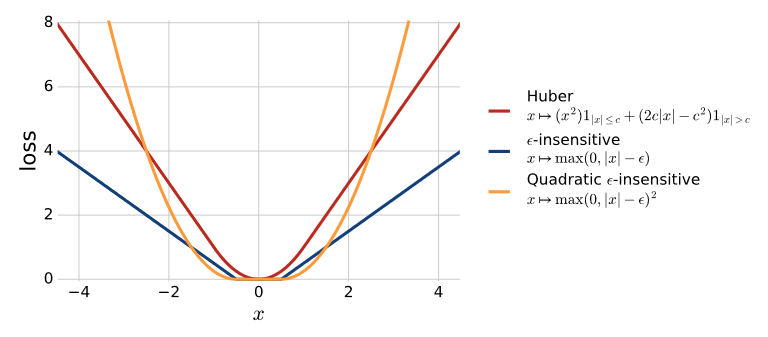
\includegraphics[width=0.8\linewidth]{Alternative loss functions with SVR.png}
    \caption{Alternative loss functions that can be used in conjunction with SVR}
    \label{fig:your_label}
\end{figure}


SVR admits several advantages: the algorithm is based on solid theoretical guarantees, the solution returned is sparse, and it allows a natural use of PDS kernels, SVR also admits favorable stability properties. However, one drawback of the algorithm is that it requires the selection of two parameters, \(C\) and \(\epsilon\). These can be selected via cross-validation, as in the case of SVMs, but this requires a relatively larger validation set. Some heuristics are often used to guide the search for their values: \(C\) is searched near the maximum value of the labels in the absence of an offset (\(b = 0\)) and for a normalized kernel, and \(\epsilon\) is chosen close to the average difference of the labels. As already discussed, the value of \(\epsilon\) determines the number of support vectors and the sparsity of the solution. Another drawback of SVR is that, as in the case of SVMs or KRR, it may be computationally expensive when dealing with large training sets. One effective solution in such cases, as for KRR, consists of approximating the kernel matrix using low-rank approximations via the Nystr{\"o}m method or the partial Cholesky decomposition. 

\section{Dual problem and quadratic programs}

The key idea is to construct a Lagrange function from the objective function (it will be called the primal objective function in the rest of this article) and the corresponding constraints, by introducing a dual set of variables. It can be shown that this function has a saddle point with respect to the primal and dual variables at the solution. For details see e.g. Mangasarian (1969), McCormick (1983), and Vanderbei (1997) and the explanations in Section 5.2. We proceed as follows:

\[
L= \frac{1}{2} \|w\|^2 + C \sum_{i=1}^{m} (\xi_i + \xi_i^*) - \sum_{i=1}^{m} (\eta_i \xi_i + \eta_i^* \xi_i^*) - \sum_{i=1}^{m} \alpha_i (\epsilon + \xi_i - y_i + \langle w, x_i \rangle + b) - \sum_{i=1}^{m} \alpha_i^* (\epsilon + \xi_i^* + y_i - \langle w, x_i \rangle - b)
\]

Here \(L\) is the Lagrangian and \(\eta_i\), \(\eta_i^*\), \(\alpha_i\), \(\alpha_i^*\) are Lagrange multipliers. Hence the dual variables in (5) have to satisfy positivity constraints, i.e.
\[
\alpha_i^*, \eta_i^* \geq 0.
\]

Note that by \(\alpha_i^*\), we refer to \(\alpha_i\) and \(\alpha_i^*\).

It follows from the saddle point condition that the partial derivatives of \(L\) with respect to the primal variables (\(w\), \(b\), \(\xi_i\), \(\xi_i^*\)) have to vanish for optimality.

\[
\frac{\partial L}{\partial b} = \sum_{i=1}^{m} (\alpha_i^* - \alpha_i) = 0
\]

\[
\frac{\partial L}{\partial w} = w - \sum_{i=1}^{m} (\alpha_i - \alpha_i^*)x_i = 0
\]

\[
\frac{\partial L}{\partial \xi_i} = C - \alpha_i^* - \eta_i^* = 0
\]

Substituting (7), (8), and (9) into (5) yields the dual optimization problem:
\[
\begin{aligned}
&\text{maximize} && 
-\frac{1}{2} \sum_{i, j=1}^{m} (\alpha_i - \alpha_i^*)(\alpha_j - \alpha_j^*) \langle x_i, x_j \rangle -\epsilon \sum_{i=1}^{m} (\alpha_i + \alpha_i^*) + \sum_{i=1}^{m} y_i (\alpha_i - \alpha_i^*) \\
&\text{subject to} && \sum_{i=1}^{m} (\alpha_i - \alpha_i^*) = 0 \text{ and } 0 \leq \alpha_i, \alpha_i^* \leq C
\end{aligned}
\]
In deriving (10) we already eliminated the dual variables $\eta_i, \eta_i^*$ through condition (9) which can be reformulated as $\eta_i^* = C - \alpha_i^*$. Equation (8) can be rewritten as $w = \sum_{i=1}^{m} (\alpha_i - \alpha_i^*)x_i$, thus $f(x) = \sum_{i=1}^{m} (\alpha_i - \alpha_i^*)\langle x_i, x \rangle + b$. This is the so-called Support Vector expansion, i.e. $w$ can be completely described as a linear combination of the training patterns $x_i$. In a sense, the complexity of a function’s representation by SVs is independent of the dimensionality of the input space $X$, and depends only on the number of SVs. Moreover, note that the complete algorithm can be described in terms of dot products between the data. Even when evaluating $f(x)$ we need not compute $w$ explicitly. These observations will come in handy for the formulation of a nonlinear extension.

\section{Computing \(b\)}

So far we neglected the issue of computing \(b\). The latter can be done by exploiting the so called Karush–Kuhn–Tucker (KKT) conditions \cite{karush1939minima,kuhn1951nonlinear}. These state that at the point of the solution the product between dual variables and constraints has to vanish:
\[
\begin{aligned}
\alpha_i (\epsilon + \xi_i - y_i + \langle w, x_i \rangle + b) &= 0 \quad &(12) \\
\alpha_i^* (\epsilon + \xi_i^* + y_i - \langle w, x_i \rangle - b) &= 0 \quad &(12') \\
(C - \alpha_i)\xi_i &= 0 \quad &(13) \\
(C - \alpha_i^*)\xi_i^* &= 0 \quad &(13')
\end{aligned}
\]

This allows us to make several useful conclusions. Firstly only samples \((x_i , y_i )\) with corresponding \(\alpha_i^* = C\) lie outside the \(\epsilon\)-insensitive tube. Secondly \(\alpha_i \alpha_i^* = 0\), i.e. there can never be a set of dual variables \(\alpha_i, \alpha_i^*\) which are both simultaneously nonzero. This allows us to conclude that
\[
\begin{aligned}
\epsilon - y_i + \langle w, x_i \rangle + b &\geq 0 \quad \text{and} \quad \xi_i = 0 && \text{if } \alpha_i < C \quad &(14) \\
\epsilon - y_i + \langle w, x_i \rangle + b &\leq 0 \quad \text{if } \alpha_i > 0 \quad &(15)
\end{aligned}
\]

In conjunction with an analogous analysis on \(\alpha_i^*\) we have
\[
\max\{-\epsilon + y_i - \langle w, x_i \rangle \,|\, \alpha_i < C \text{ or } \alpha_i^* > 0\} \leq b \leq \min\{-\epsilon + y_i - \langle w, x_i \rangle \,|\, \alpha_i > 0 \text{ or } \alpha_i^* < C\} \quad (16)
\]
If some \(\alpha_i^* \in (0,C)\) the inequalities become equalities. See also Keerthi et al. for further means of choosing \(b\).

Another way of computing \(b\) will be discussed in the context of interior point optimization (cf. Section 5). There \(b\) turns out to be a by-product of the optimization process. Further considerations shall be deferred to the corresponding section. See also Keerthi et al. for further methods to compute the constant offset.

A final note has to be made regarding the sparsity of the SV expansion. From (12) it follows that only for \(|f(x_i) - y_i| \geq \epsilon\) the Lagrange multipliers may be nonzero, or in other words, for all samples inside the \(\epsilon\)-tube (i.e. the shaded region in Fig. 1) the \(\alpha_i, \alpha_i^*\) vanish: for \(|f(x_i) - y_i| < \epsilon\) the second factor in (12) is nonzero, hence \(\alpha_i, \alpha_i^*\) has to be zero such that the KKT conditions are satisfied. Therefore we have a sparse expansion of \(w\) in terms of \(x_i\) (i.e. we do not need all \(x_i\) to describe \(w\)). The examples that come with nonvanishing coefficients are called Support Vectors.

\section{Kernels}

\subsection{Nonlinearity by Preprocessing}

The next step is to make the SV algorithm nonlinear. This, for instance, could be achieved by simply preprocessing the training patterns \(x_i\) by a map \(\phi : X \rightarrow F\) into some feature space \(F\), as described in Aizerman, Braverman and Rozono'er (1964) and Nilsson (1965) and then applying the standard SV regression algorithm. Let us have a brief look at an example given in Vapnik (1995).

\textbf{Example 1 (Quadratic features in \(\mathbb{R}^2\)):} Consider the map \(\phi : \mathbb{R}^2 \rightarrow \mathbb{R}^3\) with \(\phi(x_1, x_2) = (x_1^2, \sqrt{2}x_1x_2, x_2^2)\). It is understood that the subscripts in this case refer to the components of \(x \in \mathbb{R}^2\). Training a linear SV machine on the preprocessed features would yield a quadratic function.

While this approach seems reasonable in the particular example above, it can easily become computationally infeasible for both polynomial features of higher order and higher dimensionality, as the number of different monomial features of degree \(p\) is \({d+p-1 \choose p}\), where \(d = \text{dim}(X)\). Typical values for OCR tasks (with good performance) are \(p = 7\), \(d = 28 \times 28 = 784\), corresponding to approximately \(3.7 \times 10^{16}\) features.

\subsection{Implicit Mapping via Kernels}

Clearly this approach is not feasible and we have to find a computationally cheaper way. The key observation is that for the feature map in example 2.1 leads to:

\(\langle (x_1^2, \sqrt{2}x_1x_2, x_2^2), (x'_1^2, \sqrt{2}x'_1x'_2, x'_2^2) \rangle = \langle x, x' \rangle^2\)

As noted in the previous section, the SV algorithm only depends on dot products between patterns \(x_i\). Hence it suffices to know \(k(x, x') := \langle \phi(x), \phi(x') \rangle\) rather than \(\phi\) explicitly which allows us to restate the SV optimization problem:
\[
\begin{aligned}
&\text{maximize} \quad -\frac{1}{2} \sum_{i, j=1}^{n} (\alpha_i - \alpha_i^*)(\alpha_j - \alpha_j^*) k(x_i, x_j) - \varepsilon \sum_{i=1}^{n} (\alpha_i + \alpha_i^*) + \sum_{i=1}^{n} y_i (\alpha_i - \alpha_i^*) \\
&\text{subject to} \quad \sum_{i=1}^{n} (\alpha_i - \alpha_i^*) = 0 \quad \text{and} \quad 0 \leq \alpha_i, \alpha_i^* \leq C.
\end{aligned}
\]

Likewise, the expansion of \(f\) may be written as:
\[
w = \sum_{i=1}^{n} (\alpha_i - \alpha_i^*) \phi(x_i) \quad \text{and} \quad f(x) = \sum_{i=1}^{n} (\alpha_i - \alpha_i^*) k(x_i, x) + b.
\]

The difference to the linear case is that \(w\) is no longer given explicitly. Also, note that in the nonlinear setting, the optimization problem corresponds to finding the flattest function in feature space, not in input space.

\subsection{Conditions for Kernels}

The question that arises now is, which functions \(k(x, x')\) correspond to a dot product in some feature space \(F\). The following theorem characterizes these functions (defined on \(X\)).

\textbf{Theorem 2 (Mercer 1909).} Suppose \(k \in L_{\infty}(X^2)\) such that the integral operator \(T_k : L_2(X) \rightarrow L_2(X)\), defined as 
\[
T_k f(\cdot) = \int_X k(\cdot, x) f(x) \, d\mu(x)
\]
(here \(\mu\) denotes a measure on \(X\) with \(\mu(X)\) finite and \(\text{supp}(\mu) = X\), is positive. Let \(\psi_j \in L_2(X)\) be the eigenfunction of \(T_k\) associated with the eigenvalue \(\lambda_j \neq 0\) and normalized such that \(\|\psi_j\|_{L_2} = 1\) and let \(\overline{\psi_j}\) denote its complex conjugate. Then:

1. \(\lambda_j(T) \geq 0\) for all \(j \in \mathbb{N}\).

2. \(k(x, x') = \sum_{j \in \mathbb{N}} \lambda_j \psi_j(x) \overline{\psi_j}(x')\) holds for almost all \((x, x')\), where the series converges absolutely and uniformly for almost all \((x, x')\).

Less formally speaking, this theorem means that if
\[
\int_{XxX} k(x, x') f(x) f(x') \, dx dx' \geq 0 \ \ \forall f \in L_2(X) 
\]
holds, we can write \(k(x, x')\) as a dot product in some feature space. From this condition, we can conclude some simple rules for compositions of kernels, which then also satisfy Mercer's condition (Scholkopf, Burges and Smola 1999a). In the following, we will call such functions k admissible SV kernels.

\textbf{Corollary 3 (Positive linear combinations of kernels)}

Denote by \(k_1, k_2\) admissible SV kernels and \(c_1, c_2 \geq 0\), then
\[
k(x, x') := c_1k_1(x, x') + c_2k_2(x, x')
\]

is an admissible kernel. This follows directly from \((21)\) by virtue of the linearity of integrals. More generally, one can show that the set of admissible kernels forms a convex cone, closed in the topology of pointwise convergence (Berg, Christensen and Ressel 1984).

\textbf{Corollary 4 (Integrals of kernels)}

Let \(s(x, x')\) be a function on \(X \times X\) such that
\[
k(x, x') := \int_X s(x, z)s(x', z) \, dz
\]

exists. Then \(k\) is an admissible SV kernel. This can be shown directly from \((21)\) and \((23)\) by rearranging the order of integration. We now state a necessary and sufficient condition for translation invariant kernels, i.e. \(k(x, x') := k(x - x')\) as derived in Smola, Sch\"olkopf and M\"uller (1998c).

\textbf{Theorem 5 (Products of kernels)}

Denote by \(k_1\) and \(k_2\) admissible SV kernels, then
\[
k(x, x') := k_1(x, x')k_2(x, x')
\]

is an admissible kernel. This can be seen by an application of the "expansion part" of Mercer's theorem to the kernels \(k_1\) and \(k_2\) and observing that each term in the double sum
\[
\sum_{i, j} \lambda_{i}^1 \lambda_{j}^2 \psi_{i}^1(x) \psi_{i}^1(x') \psi_{j}^2(x) \psi_{j}^2(x')
\]

gives rise to a positive coefficient when checking \((21)\).

\textbf{Theorem 6 (Smola, Sch\"olkopf and M\"uller 1998c)}

A translation invariant kernel \(k(x, x') = k(x - x')\) is an admissible SV kernel if and only if the Fourier transform
\[
F[k](\omega) = (2\pi)^{-d/2} \int_X e^{-i \langle \omega, x \rangle} k(x) \, dx
\]

is nonnegative.

We will give a proof and some additional explanations to this theorem in Section 7. It follows from interpolation theory (Micchelli 1986) and the theory of regularization networks (Girosi, Jones and Poggio 1993). For kernels of the dot-product type, i.e. \(k(x, x') = k(\langle x, x' \rangle)\), there exist sufficient conditions for being admissible.

\textbf{Theorem 7 (Burges 1999)}

Any kernel of dot-product type \(k(x, x') = k(\langle x, x' \rangle)\) has to satisfy
\[
k(\xi) \geq 0, \quad \partial_\xi k(\xi) \geq 0, \quad \text{and} \quad \partial_\xi k(\xi) + \xi \partial^2_\xi k(\xi) \geq 0
\]

for any \(\xi \geq 0\) in order to be an admissible SV kernel. Note that the conditions in Theorem 7 are only necessary but not sufficient.

\textbf{Theorem 8 (Schoenberg 1942)}

A kernel of dot-product type \(k(x, x') = k(\langle x, x' \rangle)\) defined on an infinite dimensional Hilbert space, with a power series expansion
\[
k(t) = \sum_{n=0}^\infty a_n t^n
\]

is admissible if and only if all \(a_n \geq 0\). A slightly weaker condition applies for finite dimensional spaces. For further details see Berg, Christensen and Ressel (1984) and Smola, O´ va´ri and Williamson (2001).

\textbf{Examples}

In Sch¨olkopf, Smola and M¨uller (1998b) it has been shown, by explicitly computing the mapping, that homogeneous polynomial kernels \(k\) with \(p \in \mathbb{N}\) and
\[
k(x, x') = \langle x, x' \rangle^p
\]

are suitable SV kernels (cf. Poggio 1975). From this observation one can conclude immediately (Boser, Guyon and Vapnik 1992, Vapnik 1995) that kernels of the type
\[
k(x, x') = (\langle x, x' \rangle + c)^p
\]

i.e. inhomogeneous polynomial kernels with \(p \in \mathbb{N}\), \(c \geq 0\) are admissible, too: rewrite \(k\) as a sum of homogeneous kernels and apply Corollary 3.

Another kernel, that might seem appealing due to its resemblance to Neural Networks is the hyperbolic tangent kernel
\[
k(x, x') = \tanh(\theta + \kappa \langle x, x' \rangle).
\]

By applying Theorem 8 one can check that this kernel does not actually satisfy Mercer’s condition (Ovari 2000). Curiously, the kernel has been successfully used in practice; cf. Scholkopf (1997) for a discussion of the reasons.

Translation invariant kernels \(k(x, x') = k(x - x')\) are quite widespread. It was shown in Aizerman, Braverman and Rozono´er (1964), Micchelli (1986) and Boser, Guyon and Vapnik (1992) that
\[
k(x, x') = e^{-\frac{\|x-x'\|^2}{2\sigma^2}}
\]

is an admissible SV kernel. Moreover one can show (Smola 1996, Vapnik, Golowich and Smola 1997) that \(\mathbb{1}_X\) denotes the indicator function on the set \(X\) and \(\otimes\) the convolution operation)
\[
k(x, x') = B_{2n+1}(\|x - x'\|) \quad \text{with} \quad B_k := k \otimes_{i=1}^k 1_{\left[-\frac{1}{2}, \frac{1}{2}\right]}
\]
B-splines of order \(2n + 1\), defined by the \(2n + 1\) convolution of the unit interval, are also admissible. We shall postpone further considerations to Section 9 where the connection to regularization operators will be pointed out in more detail.

\section{Cost functions}
So far the SV algorithm for regression may seem rather strange and hardly related to other existing methods of function estimation (e.g. Huber 1981, Stone 1985, H¨ardle 1990, Hastie and Tibshirani 1990, Wahba 1990). However, once cast into a more standard mathematical notation, we will observe the connections to previous work. For the sake of simplicity we will, again, only consider the linear case, as extensions to the nonlinear one are straightforward by using the kernel method described in the previous chapter.

\subsection{The risk functional}
Let us for a moment go back to the case we had earlier. There, we had some training data $X := \{(x_1, y_1), \ldots, (x_n, y_n)\} \subset X \times \mathbb{R}$. We will assume now, that this training set has been drawn iid
(independent and identically distributed) from some probability distribution $P(x, y)$. Our goal will be to find a function $f$ minimizing the expected risk (cf. Vapnik 1982)
\[ R[ f ] = \int c(x, y, f (x)) \, dP(x, y) \]

$(c(x, y, f (x))$ denotes a cost function determining how we will penalize estimation errors) based on the empirical data $X$. Given that we do not know the distribution $P(x, y)$ we can only use $X$ for estimating a function $f$ that minimizes $R[ f ]$. A possible approximation consists in replacing the integration by the empirical estimate, to get the so called empirical risk functional
\[ R_{\text{emp}}[ f ] := \frac{1}{n} \sum_{i=1}^{n} c(x_i, y_i, f (x_i )) \]

A first attempt would be to find the empirical risk minimizer $f_0 := \arg \min_{f \in H} R_{\text{emp}}[ f ]$ for some function class $H$. However, if $H$ is very rich, i.e. its “capacity” is very high, as for instance when dealing with few data in very high-dimensional spaces, this may not be a good idea, as it will lead to overfitting and thus bad generalization properties. Hence one should add a capacity control term, in the SV case $\|w\|^2$, which leads to the regularized
risk functional (Tikhonov and Arsenin 1977, Morozov 1984, Vapnik 1982)
\[ R_{\text{reg}}[ f ] := R_{\text{emp}}[ f ] + \frac{\lambda}{2} \|w\|^2 \]

where $\lambda > 0$ is a so called regularization constant. Many algorithms like regularization networks (Girosi, Jones and Poggio 1993) or neural networks with weight decay networks (e.g. Bishop 1995) minimize an expression similar to (35).

\subsection{Maximum likelihood and density models}
The standard setting in the SV case is, as already mentioned in
Section 1.2, the $\epsilon$-insensitive loss
\[ c(x, y, f (x)) = |y - f (x)|_{\epsilon}. \]

It is straightforward to show that minimizing (35) with the particular loss function of (36) is equivalent to minimizing (3), the only difference being that $C = \frac{1}{(\lambda l)}$.

Loss functions such like $|y - f (x)|^p_\epsilon$ with $p > 1$ may not be desirable, as the superlinear increase leads to a loss of the robustness properties of the estimator (Huber 1981): in those cases the derivative of the cost function grows without bound. For $p < 1$, on the other hand, $c$ becomes nonconvex.

For the case of $c(x, y, f (x)) = (y - f (x))^2$ we recover the least mean squares fit approach, which, unlike the standard SV loss function, leads to a matrix inversion instead of a quadratic programming problem.

The question is which cost function should be used in (35). On
the one hand we will want to avoid a very complicated function $c$ as this may lead to difficult optimization problems. On the other hand one should use that particular cost function that suits the problem best. Moreover, under the assumption that the samples were generated by an underlying functional dependency plus additive noise, i.e. $y_i = f_{\text{true}}(x_i) + \xi_i$ with density $p(\xi)$, then the optimal cost function in a maximum likelihood sense is
\[ c(x, y, f (x)) = -\log p(y - f (x)). \]

This can be seen as follows. The likelihood of an estimate
\[ X_f := \{(x_1, f (x_1)), \ldots, (x_n, f (x_n))\} \]
for additive noise and iid data is
\[p(X f | X) = \prod_{i=1}^n p(f(x_i) | (x_i, y_i)) = \prod_{i=1}^n p(y_i - f(x_i))\].

Maximizing $P(X_f |X)$ is equivalent to minimizing $-\log P(X_f |X)$. By using (35) we get
\[ -\log P(X_f |X) = \sum_{i=1}^{n} c(x_i, y_i, f (x_i)). \]

However, the cost function resulting from this reasoning might be nonconvex. In this case one would have to find a convex proxy in order to deal with the situation efficiently (i.e. to find an efficient implementation of the corresponding optimization problem).

If, on the other hand, we are given a specific cost function from a real world problem, one should try to find as close a proxy to this cost function as possible, as it is the performance wrt. this particular cost function that matters ultimately.

Table 1 contains an overview over some common density models and the corresponding loss functions as defined by (35).

The only requirement we will impose on $c(x, y, f (x))$ in the
following is that for fixed $x$ and $y$ we have convexity in $f (x)$.
This requirement is made, as we want to ensure the existence and
uniqueness (for strict convexity) of a minimum of optimization
problems (Fletcher 1989).

\subsection{Solving the equations}
For the sake of simplicity we will additionally assume $c$ to be symmetric and to have (at most) two (for symmetry) discontinuities at $\pm\epsilon$, $\epsilon \geq 0$ in the first derivative, and to be zero in the interval $[-\epsilon, \epsilon]$. All loss functions from Table 1 belong to this class. Hence $c$ will take on the following form.
\[ c(x, y, f (x)) = \tilde{c}(|y - f (x)|\epsilon) \tag{41} \]

Note the similarity to Vapnik’s $\epsilon$-insensitive loss. It is rather straightforward to extend this special choice to more general convex cost functions. For nonzero cost functions in the interval $[-\epsilon, \epsilon]$ use an additional pair of slack variables. Moreover we might choose different cost functions $\tilde{c}_i$, $\tilde{c}^*_i$ and different values of $\epsilon_i$, $\epsilon^*_i$ for each sample. At the expense of additional Lagrange multipliers in the dual formulation additional discontinuities also can be taken care of. Analogously to (3) we arrive at a convex minimization problem (Smola and Sch\"olkopf 1998a).

To simplify notation we will stick to the one of (3) and use $C$ instead of normalizing by $\lambda$ and \({l} \)
\[
\begin{aligned}
\text{minimize} \quad & \frac{1}{2} \|w\|^2 + C \sum_{i=1}^{n} \left(c\tilde{(\xi_i)} + c\tilde{(\xi^*_i)}\right) \\
\text{subject to} \quad & 
\begin{cases}
    y_i - \langle w, x_i \rangle - b \leq \epsilon + \xi_i, \\
    \langle w, x_i \rangle + b - y_i \leq \epsilon + \xi^*_i, \\
    \xi_i, \xi^*_i \geq 0
\end{cases}
\end{aligned}
\tag{42}
\]

Again, by standard Lagrange multiplier techniques, exactly in the same manner as in the $|\cdot|_\epsilon$ case, one can compute the dual optimization problem (the main difference is that the slack variable terms $c\tilde{(\xi)}$ now have nonvanishing derivatives). We will omit the indices $i$ and $*$, where applicable to avoid tedious notation. This yields:

\[
\begin{aligned}
\text{maximize} \quad & \frac{1}{2} \sum_{i,j=1}^{n} (\alpha_i - \alpha^*_i)(\alpha_j - \alpha^*_j) \langle x_i, x_j \rangle + \sum_{i=1}^{n} y_i(\alpha_i - \alpha^*_i) - \epsilon(\alpha_i + \alpha^*_i) + C\sum_{i=1}^{n} T(\xi_i) + T(\xi^*_i) \\
\end{aligned}
\]
\[
\begin{aligned}
\text{where} \begin{cases} w = \sum_{i=1}^{n} (\alpha_i - \alpha^*_i) x_i \\
T(\xi) := c\tilde{(\xi)} - \xi \cdot \partial_\xi c\tilde{(\xi)}
\end{cases}
\end{aligned}
\tag{43}
\]
\[
\begin{aligned}
\text{subject to: }
\begin{cases}
    \sum_{i=1}^{n} (\alpha_i - \alpha^*_i) = 0, \\
    \alpha \leq C \partial_\xi c\tilde{(\xi)}, \\
    \xi = \inf \{\xi | C \partial_\xi c\tilde{(\xi)} \geq \alpha\}, \\
    \alpha, \xi \geq 0
\end{cases}
\end{aligned}
\]

Note that the maximum slope of $c\tilde{(\xi)}$ determines the region of feasibility of $\alpha$, i.e., \\$s = \sup_{\xi \in \mathbb{R}^+} \partial_\xi c\tilde{(\xi)} < \infty$ \ leads to compact intervals $[0, Cs]$ for $\alpha$. This means that the influence of a single pattern is bounded, leading to robust estimators (Huber 1972). One can also observe experimentally that the performance of a SV machine depends significantly on the cost function used (M¨uller et al. 1997, Smola, Sch¨olkopf and M¨uller 1998b).

A cautionary remark is necessary regarding the use of cost functions other than the $\epsilon$-insensitive one. Unless $\epsilon = 0$ we will lose the advantage of a sparse decomposition. This may be acceptable in the case of few data, but will render the prediction step extremely slow otherwise. Hence one will have to trade off a potential loss in prediction accuracy with faster predictions. Note, however, that also a reduced set algorithm like in Burges (1996), Burges and Sch¨olkopf (1997) and Sch¨olkopf et al. (1999b) or sparse decomposition techniques (Smola and Sch¨olkopf 2000) could be applied to address this issue. In a Bayesian setting, Tipping (2000) has recently shown how an $L_2$ cost function can be used without sacrificing sparsity.

\section{Optimization algorithms}
While there has been a large number of implementations of SV algorithms in the past years, we focus on a few algorithms which will be presented in greater detail. This selection is somewhat biased, as it contains these algorithms the authors are most familiar with. However, we think that this overview contains some
of the most effective ones and will be useful for practitioners who would like to actually code a SV machine by themselves. But before doing so we will briefly cover major optimization packages and strategies.

\subsection{Interior point algorithms}

In a nutshell the idea of an interior point algorithm is to compute the dual of the optimization problem (in our case the dual dual of $R_{\text{reg}}[ f ]$) and solve both primal and dual simultaneously. This is done by only gradually enforcing the KKT conditions to iteratively find a feasible solution and to use the duality gap between primal and dual objective function to determine the quality of the current set of variables. The special flavour of algorithm we will describe is primal-dual path-following (Vanderbei 1994).

In order to avoid tedious notation we will consider the slightly more general problem and specialize the result to the SVM later. It is understood that unless stated otherwise, variables like $\alpha$ denote vectors and $\alpha_i$ denotes its $i$-th component.
\[
\begin{aligned}
    &\text{minimize} && \frac{1}{2} q(\alpha) + \langle c, \alpha \rangle \\
    &\text{subject to} && A\alpha = b \text{ and } l \leq \alpha \leq u
\end{aligned}
\]

with $c, \alpha, l, u \in \mathbb{R}^n$, $A \in \mathbb{R}^{n \times m}$, $b \in \mathbb{R}^m$, the inequalities between vectors holding componentwise and $q(\alpha)$ being a convex function of $\alpha$. Now we will add slack variables to get rid of all inequalities but the positivity constraints. This yields:

\[
\begin{aligned}
    &\text{minimize} && \frac{1}{2} q(\alpha) + \langle c, \alpha \rangle \\
    &\text{subject to} && A\alpha = b, \ \alpha - g = l, \ \alpha + t = u, \\
    &&& g, t \geq 0, \ \alpha \text{ free}
\end{aligned}
\]

The dual of (51) is
\[
\begin{aligned}
    &\text{maximize} && \frac{1}{2} \left(q(\alpha) - \langle \partial q(\alpha), \alpha \rangle\right) + \langle b, y \rangle + \langle l, z \rangle - \langle u, s \rangle \\
    &\text{subject to} && \frac{1}{2} \partial q(\alpha) + c - (Ay) + s = z, \ s, z \geq 0, \ y \text{ free}
\end{aligned}
\]

Moreover we get the KKT conditions, namely $g_i z_i = 0$ and $s_i t_i = 0$ for all $i \in [1 . . . n]$.

A necessary and sufficient condition for the optimal solution is that the primal/dual variables satisfy both the feasibility conditions of (51) and (52) and the KKT conditions (53). We proceed to solve (51)–(53) iteratively.

\subsection{Useful tricks}

Before proceeding to further algorithms for quadratic optimization let us briefly mention some useful tricks that can be applied to all algorithms described subsequently and may have significant impact despite their simplicity. They are in part derived from ideas of the interior-point approach.

\subsubsection{Training with different regularization parameters}

For several reasons (model selection, controlling the number of support vectors, etc.) it may happen that one has to train a SV machine with different regularization parameters \(C\), but otherwise rather identical settings. If the parameters \(C_{\text{new}} = \tau C_{\text{old}}\) is not too different it is advantageous to use the rescaled values of the Lagrange multipliers (i.e. \(\alpha_i, \alpha_i^*\)) as a starting point for the new optimization problem. Rescaling is necessary to satisfy the modified constraints. One gets
\[
\alpha_{\text{new}} = \tau \alpha_{\text{old}} \quad \text{and likewise} \quad b_{\text{new}} = \tau b_{\text{old}}. \quad (54)
\]

Assuming that the (dominant) convex part \(q(\alpha)\) of the primal objective is quadratic, the \(q\) scales with \(\tau^2\) whereas the linear part scales with \(\tau\). However, since the linear term dominates the objective function, the rescaled values are still a better starting point than \(\alpha = 0\). In practice a speedup of approximately 95\% of the overall training time can be observed when using the sequential minimization algorithm. A similar reasoning can be applied when retraining with the same regularization parameter but different (yet similar) width parameters of the kernel function.

\subsubsection{Monitoring convergence via the feasibility gap}

In the case of both primal and dual feasible variables, the following connection between primal and dual objective function holds:
\[
\text{Dual Obj.} = \text{Primal Obj.} - \sum_i (g_i z_i + s_i t_i). \quad (55)
\]

This can be seen immediately by the construction of the Lagrange function. In Regression Estimation (with the \(\epsilon\)-insensitive loss function) one obtains for
\[
\begin{aligned}
&\sum_i g_i z_i + s_i t_i
& = \sum_i \max [ \left(0, f(x_i) - (y_i + \epsilon_i)\right)(C - \alpha_i^*) - \min \left(0, f(x_i) - (y_i + \epsilon_i)\right)\alpha_i^* \center + \max \left(0, (y_i - \epsilon_i^*) - f(x_i)\right)(C - \alpha_i) - \min \left(0, (y_i - \epsilon_i^*) - f(x_i)\right)\alpha_i ]
\end{aligned}
\]

Thus convergence with respect to the point of the solution can be expressed in terms of the duality gap. An effective stopping rule is to require

\[
\frac{\sum_i g_i z_i + s_i t_i}{|\text{Primal Objective}| + 1} \leq \text{\(\epsilon_{\text{tol}}\)} \quad (57)
\]

for some precision \(\epsilon_{\text{tol}}\). This condition is much in the spirit of primal dual interior point path following algorithms, where convergence is measured in terms of the number of significant figures (which would be the decimal logarithm of (57)), a convention that will also be adopted in the subsequent parts of this exposition.

\subsection{Regularization}

So far we were not concerned about the specific properties of the map \( \phi \) into feature space and used it only as a convenient trick to construct nonlinear regression functions. In some cases the map was just given implicitly by the kernel, hence the map itself and many of its properties have been neglected. A deeper understanding of the kernel map would also be useful in choosing appropriate kernels for a specific task (e.g. by incorporating prior knowledge (Scholkopf1998a). Finally the feature map seems to defy the curse of dimensionality (Bellman1961) by making problems seemingly easier yet reliable via a map into some even higher dimensional space.

In this section, we focus on the connections between SV methods and previous techniques like Regularization Networks (RNs) (Girosi1993). In particular, we will show that SV machines are essentially Regularization Networks (RN) with a clever choice of cost functions and that the kernels are Green’s function of the corresponding regularization operators. For a full exposition of the subject, the reader is referred to (Smola1998c).

\subsubsection{Regularization networks}

Let us briefly review the basic concepts of RNs. As in (35) we minimize a regularized risk functional. However, rather than enforcing flatness in feature space we try to optimize some smoothness criterion for the function in input space. Thus we get
\[
R_{\text{reg}}[ f ] := R_{\text{emp}}[ f ] + \lambda \frac{1}{2} \| Pf \|^2. \quad (64)
\]

Here \(P\) denotes a regularization operator in the sense of Tikhonov and Arsenin (1977), i.e. \(P\) is a positive semidefinite operator mapping from the Hilbert space \(H\) of functions \(f\) under consideration to a dot product space \(D\) such that the expression \(\langle Pf, Pg \rangle\) is well defined for \(f, g \in H\). For instance by choosing a suitable operator that penalizes large variations of \(f\) one can reduce the well–known overfitting effect. Another possible setting also might be an operator \(P\) mapping from \(L^2(\mathbb{R}^n)\) into some Reproducing Kernel Hilbert Space (RKHS) (Aronszajn1950, Kimeldorf1971, Saitoh1988, Scholkopf1997, Girosi1998).

Using an expansion of \(f\) in terms of some symmetric function \(k(x_i, x_j)\) (note here, that \(k\) need not fulfill Mercer’s condition and can be chosen arbitrarily since it is not used to define a regularization term),
\[
f(x) = \sum_{i=1}^N \alpha_i k(x_i, x) + b, \quad (65)
\]

and the \(\epsilon\)-insensitive cost function, this leads to a quadratic programming problem similar to the one for SVs. Using
\[
D_{ij} := \langle (Pk)(x_i, \cdot), (Pk)(x_j, \cdot) \rangle, \quad (66)
\]

we get \(\alpha = D^{-1}K(\beta - \beta^*)\), with \(\beta, \beta^*\) being the solution of
\[
\begin{aligned}
&\text{minimize} && \frac{1}{2} (\beta^* - \beta)^T K D^{-1} K (\beta^* - \beta) - (\beta^* - \beta)^T y - \epsilon \sum_{i=1}^N (\beta_i + \beta^*_i) \\
&\text{subject to} && \sum_{i=1}^N (\beta_i - \beta^*_i) = 0 \quad \text{and} \quad \beta_i, \beta^*_i \in [0,C]. \quad (67)
\end{aligned}
\]

Unfortunately, this setting of the problem does not preserve sparsity in terms of the coefficients, as a potentially sparse decomposition in terms of \(\beta_i\) and \(\beta^*_i\) is spoiled by \(D^{-1}K\), which is not in general diagonal.

\subsubsection{Green’s functions}

Comparing (10) with (67) leads to the question of whether and under which condition the two methods might be equivalent and therefore also under which conditions regularization networks might lead to sparse decompositions, i.e. only a few of the expansion coefficients \(\alpha_i\) in \(f\) would differ from zero. A sufficient condition is \(D = K\) and thus \(KD^{-1}K = K\) (if \(K\) does not have full rank we only need that \(KD^{-1}K = K\) holds on the image of \(K\)):
\[
k(x_i, x_j) = \langle (Pk)(x_i, \cdot), (Pk)(x_j, \cdot) \rangle. \quad (68)
\]

Our goal now is to solve the following two problems:

1. Given a regularization operator \(P\), find a kernel \(k\) such that a SV machine using \(k\) will not only enforce flatness in feature space, but also correspond to minimizing a regularized risk functional with \(P\) as regularizer.

2. Given an SV kernel \(k\), find a regularization operator \(P\) such that a SV machine using this kernel can be viewed as a Regularization Network using \(P\).

These two problems can be solved by employing the concept of Green’s functions as described in (Girosi1993). These functions were introduced for the purpose of solving differential equations. In our context it is sufficient to know that the Green’s functions \(G_{x_i}(x)\) of \(P^*P\) satisfy
\[
(P^*PG_{x_i})(x) = \delta_{x_i}(x). \quad (69)
\]

Here, \(\delta_{x_i}(x)\) is the \(\delta\)-distribution (not to be confused with the Kronecker symbol \(\delta_{ij}\)) which has the property that \(\langle f, \delta_{x_i} \rangle = f(x_i)\).

The relationship between kernels and regularization operators is formalized in the following proposition:

\textbf{Proposition 1} (Smola1998b). Let \(P\) be a regularization operator, and \(G\) be the Green’s function of \(P^*P\). Then \(G\) is a Mercer Kernel such that \(D = K\). SV machines using \(G\) minimize risk functional (64) with \(P\) as regularization operator.

In the following we will exploit this relationship in both ways: to compute Green’s functions for a given regularization operator \(P\) and to infer the regularizer, given a kernel \(k\).

\subsubsection{Translation invariant kernels}

Let us now more specifically consider regularization operators \(\hat{P}\) that may be written as multiplications in Fourier space:
\[
\langle Pf, Pg \rangle = \frac{1}{{(2\pi)^{n/2}}} \int_{\Omega} \frac{\overline{\tilde{f}(\omega)}\tilde{g}(\omega)} {{P}(\omega)} d\omega \quad (70)
\]

with \(\tilde{f}(\omega)\) denoting the Fourier transform of \(f(x)\), and \({P}(\omega) = {P}(-\omega)\) real valued, nonnegative and converging to 0 for \(|\omega| \to \infty\) and \(\langle \cdot, \cdot \rangle := \text{supp}[{P}(\omega)]\). Small values of \({P}(\omega)\) correspond to a strong attenuation of the corresponding frequencies. Hence small values of \({P}(\omega)\) for large \(\omega\) are desirable since high frequency components of \(\hat{f}\) correspond to rapid changes in \(f\). \({P}(\omega)\) describes the filter properties of \(P^*P\). Note that no attenuation takes place for \({P}(\omega) = 0\) as these frequencies have been excluded from the integration domain.

For regularization operators defined in Fourier Space by (70) one can show by exploiting \({P}(\omega) = {P}(-\omega) = {P}(\omega)\) that:
\[
G(x_i, x) = \frac{1}{{(2\pi)^{n/2}}} \int_{\mathcal{R}^n} e^{i\omega(x_i - x)}{P}(\omega) d\omega \quad (71)
\]

is a corresponding Green’s function satisfying translational invariance, i.e. \(G(x_i, x_j) = G(x_i - x_j)\) and \(\hat{G}(\omega) = {P}(\omega)\) (72). This provides us with an efficient tool for analyzing SV kernels and the types of capacity control they exhibit. In fact the above is a special case of Bochner’s theorem (Bochner1959) stating that the Fourier transform of a positive measure constitutes a positive Hilbert Schmidt kernel.

\textbf{Example 2} (Gaussian kernels). Following the exposition of Yuille and Grzywacz (Yuille1988) as described in (Girosi1993), one can see that for
\[
\|P f \|_2 = \int dx \sum_{m} \frac{\sigma^{2m}}{m!2^m} (\hat{O}_m f(x))^2 \quad (73)
\]

with \(\hat{O}^{2m} = \Delta^m\) and \(\hat{O}^{2m+1} = \nabla \Delta^m\), \(\Delta\) being the Laplacian and \(\nabla\) the Gradient operator, we get Gaussian kernels (31). Moreover, we can provide an equivalent representation of \(P\) in terms of its Fourier properties, i.e. \(\hat{P}(\omega) = e^{-\sigma^2|\omega|^2/2}\) up to a multiplicative constant.

Training an SV machine with Gaussian RBF kernels (Sch¨olkopf et al. 1997) corresponds to minimizing the specific cost function with a regularization operator of type (73). Recall that (73) means that all derivatives of \(f\) are penalized (we have a pseudo-differential operator) to obtain a very smooth estimate. This also explains the good performance of SV machines in this case, as it is by no means obvious that choosing a flat function in some high dimensional space will correspond to a simple function in low dimensional space, as shown in (Smola1998c) for Dirichlet kernels.

The question that arises now is which kernel to choose. Let us think about two extreme situations.

1. Suppose we already knew the shape of the power spectrum \(Pow(\omega)\) of the function we would like to estimate. In this case we choose \(k\) such that \(\hat{k}\) matches the power spectrum (Smola1998).

2. If we happen to know very little about the given data a general smoothness assumption is a reasonable choice. Hence we might want to choose a Gaussian kernel. If computing time is important one might moreover consider kernels with compact support, e.g. using the Bq–spline kernels (cf. (32)). This choice will cause many matrix elements \(k_{ij} = k(x_i-x_j)\) to vanish.

The usual scenario will be in between the two extreme cases and we will have some limited prior knowledge available. For more information on using prior knowledge for choosing kernels (Scholkopf1998a).

\section{SVR hands on Example}
The constrained quadratic optimization problem can be solved by finding the Lagrangian. The Lagrange multipliers, or dual variables, are $\lambda$, $\lambda^*$, $\alpha$, $\alpha^*$ and are non-negative real numbers. Using the KKT conditions we have:
\[
\frac{\partial L}{\partial b} = \sum_{i=1}^{m} (\alpha_i^* - \alpha_i) = 0
\]
\[
\frac{\partial L}{\partial w} = w - \sum_{i=1}^{m} (\alpha_i - \alpha_i^*)x_i = 0
\]
\[
\frac{\partial L}{\partial \xi_i^*} = C - \alpha_i^* - \eta_i^* = 0
\]
\[
\frac{\partial L}{\partial \xi_i} = C - \alpha_i - \eta_i = 0
\]
\[
\frac{\partial L}{\partial \alpha_i^*} = y_i - w^Tx_i - \epsilon -\xi_i^* \leq 0
\]
\[
\frac{\partial L}{\partial \alpha_i} = y_i - w^Tx_i - \epsilon -\xi_i \leq 0
\]
\[
\frac{\partial L}{\partial \eta_i^*} =\sum_{i=1}^N \xi_i^* \leq 0
\]
\[
\frac{\partial L}{\partial \eta_i} =\sum_{i=1}^N \xi_i \leq 0
\]
\[
\alpha_i(-y_i + w^Tx_i - \epsilon - \xi_i) = 0
\]
\[
\alpha_i^*(y_i - w^Tx_i - \epsilon - \xi_i^*) = 0
\]
\[
\eta_i^*\xi_i^* = 0
\]
\[
\eta_i\xi_i = 0
\]

We get:
\[
w = \sum_{i=1}^N(\alpha_i^* - \alpha_i)x_i
\]

Lets consider three points (1,1), (1,-1), and (2,3). Then use SVR model to calculate w and b.
According to the dual formula, we get:
\[
\begin{aligned}
&\text{maximize}_{\alpha_i, \alpha_i^*} && 
-\frac{1}{2} \sum_{i, j=1}^{m} (\alpha_i - \alpha_i^*)(\alpha_j - \alpha_j^*) \langle x_i, x_j \rangle -\epsilon \sum_{i=1}^{m} (\alpha_i + \alpha_i^*) + \sum_{i=1}^{m} y_i (\alpha_i - \alpha_i^*) \\
&\text{subject to} && \sum_{i=1}^{m} (\alpha_i - \alpha_i^*) = 0 \text{ and } 0 \leq \alpha_i, \alpha_i^* \leq C
\end{aligned}
\]
We know that $x_1 = 1$, $y_1 = 1$, $x_2 = 1$, $y_2 = -1$, $x_3 = 2$, $y_3 = 3$.
From the initial Lagrange constraints we know that:
\[
w = \sum_{i=1}^N(\alpha_i^* - \alpha_i)x_i
\]

Therefore if we solve for $(\alpha_i^* - \alpha_i)$ we can get w. From $y_i = w^Tx_i + b$, we know that  $b = y_i - w^Tx_i$. So if we calculate w, we can calculate b.

\[
\begin{aligned}
\max_{\alpha_i, \alpha_i^*} \ \
1 \times (\alpha_1^* - \alpha_1) + (-1)\times(\alpha_2^* - \alpha_2) + 3\times(\alpha_3^* - \alpha_3) - \epsilon(\alpha_1^* + \alpha_1 + \alpha_2^* + \alpha_2 + \alpha_3^* + \alpha_3) \\
- \frac{1}{2}(\alpha_1^* - \alpha_1)(\alpha_2^* - \alpha_2)\times1\times 1 + \frac{1}{2}(\alpha_1^* - \alpha_1)(\alpha_3^* - \alpha_3)\times1\times 2 + \frac{1}{2}(\alpha_2^* - \alpha_2)(\alpha_3^* - \alpha_3)\times1\times 2
\end{aligned}
\]

We set $\epsilon = 1$
Using KKT conditions:
\[
\begin{aligned}
\frac{\partial L}{\partial \alpha_1} = -1+\epsilon+\frac{1}{2}(\alpha_2^* - \alpha_2) + (\alpha_3^* - \alpha_3) = 0 \\
\frac{\partial L}{\partial \alpha_2} = 1+\epsilon+\frac{1}{2}(\alpha_1^* - \alpha_1) + (\alpha_3^* - \alpha_3) = 0 \\
\frac{\partial L}{\partial \alpha_1} = -3+\epsilon+\frac{1}{2}(\alpha_1^* - \alpha_1) + (\alpha_2^* - \alpha_2) = 0
\end{aligned}
\]
We also have:
\[
w = \sum_{i=1}^N(\alpha_i^* - \alpha_i)x_i
\]
To simplify calculations, we use $A_1$, $A_2$, and $A_3$ instead of $(\alpha_1^* - \alpha_1)$, $(\alpha_2^* - \alpha_2)$, and $(\alpha_3^* - \alpha_3)$. Then we get:
\[
\begin{aligned}
\frac{\partial L}{\partial \alpha_1} = -1+\epsilon+\frac{1}{2}(A_2) + (A_3) = 0 \\
\frac{\partial L}{\partial \alpha_2} = 1+\epsilon+\frac{1}{2}(A_1) + (A_3) = 0 \\
\frac{\partial L}{\partial \alpha_1} = -3+\epsilon+\frac{1}{2}(A_1) + (A_2) = 0 \\
\end{aligned}
\]

\(A_1 = -2\) \ \(A_2 = -2\) \ \(A_3 = 4\) \\\\
Then we can calculate:\\
$w = -2\times1 +(-2)\times(-1) +4\times2 = -2$ \\\\
$b = 1 - (-2)\times1=3$ \\\\
Therefore the regression for these three points is: \\\\
$y = -2x+3$

\section{Conclusion}

In many cases, it may be possible to achieve similar performance with neural network methods, however, only if many parameters are optimally tuned by hand, thus depending largely on the skill of the experimenter. Certainly, SV machines are not a “silver bullet.” However, as they have only a few critical parameters (e.g. regularization and kernel width), state-of-the-art results can be achieved with relatively little effort.

\section{Appendix}
\subsection{Linear Regression}

We start with the simplest algorithm for regression known as linear regression. Let $\boldsymbol{\phi}: X \to \mathbb{R}^N$ be a feature mapping from the input space $X$ to $\mathbb{R}^N$, and consider the family of linear hypotheses:

\[
\mathcal{H} = \{x \mapsto \mathbf{w} \cdot \boldsymbol{\phi}(x) + b : \mathbf{w} \in \mathbb{R}^N, b \in \mathbb{R}\} \quad \text{(11.7)}
\]

Linear regression consists of seeking a hypothesis in $\mathcal{H}$ with the smallest empirical mean squared error. Thus, for a sample $S = \{(x_1, y_1), \ldots, (x_m, y_m)\} \in (X \times Y)^m$, the following is the corresponding optimization problem:

\[
\min_{\mathbf{w}, b} \frac{1}{m} \sum_{i=1}^{m} (\mathbf{w} \cdot \boldsymbol{\phi}(x_i) + b - y_i)^2 \quad \text{(11.8)}
\]

Figure 11.3 illustrates the algorithm in the simple case where $N = 1$. The optimization problem admits the simpler formulation:

\[
\min_{\mathbf{W}} F(\mathbf{W}) = \frac{1}{m} \|\mathbf{X} \cdot \mathbf{W} - \mathbf{Y}\|^2 \quad \text{(11.9)}
\]

using the notation $\mathbf{X} = \begin{bmatrix} \boldsymbol{\phi}(x_1) & \ldots & \boldsymbol{\phi}(x_m) \\ 1 & \ldots & 1 \end{bmatrix}$, $\mathbf{W} = \begin{bmatrix} \mathbf{w} \\ b \end{bmatrix}$, and $\mathbf{Y} = \begin{bmatrix} y_1 \\ \vdots \\ y_m \end{bmatrix}$. The objective function $F$ is convex, by composition of the convex function $u \mapsto \|u\|^2$ with the affine function $\mathbf{W} \mapsto \mathbf{X} \cdot \mathbf{W} - \mathbf{Y}$, and it is differentiable. Thus, $F$ admits a global minimum at $\mathbf{W}$ if and only if $\nabla F(\mathbf{W}) = \mathbf{0}$, that is if and only if:

\[
\frac{2}{m} \mathbf{X} \left(\mathbf{X} \cdot \mathbf{W} - \mathbf{Y}\right) = \mathbf{0} \quad \text{or} \quad \mathbf{X} \cdot \mathbf{X}^T \mathbf{W} = \mathbf{X} \cdot \mathbf{Y} \quad \text{(11.10)}
\]

When $\mathbf{X} \cdot \mathbf{X}^T$ is invertible, this equation admits a unique solution. Otherwise, the equation admits a family of solutions that can be given in terms of the pseudo-inverse of matrix $\mathbf{X} \cdot \mathbf{X}^T$ (see appendix A) by:

\[
\mathbf{W} = \left(\mathbf{X} \cdot \mathbf{X}^T\right)^{-1} \mathbf{X} \cdot \mathbf{Y} + \left(\mathbf{I} - \left(\mathbf{X} \cdot \mathbf{X}^T\right)^{-1} \mathbf{X} \cdot \mathbf{X}^T\right) \mathbf{W}_0
\]

where $\mathbf{W}_0$ is an arbitrary matrix in $\mathbb{R}^{N+1 \times N+1}$. Among these,
The solution $W = (XX>)^{-1}XY$ is the one with the minimal norm and is often preferred for that reason. Thus, we will write the solutions as:

\[
W = \begin{cases} 
      (XX^T)^{-1}XY & \text{if } XX> \text{ is invertible;} \\
      (XX^T)^\mathcal{+}XY & \text{otherwise.}
   \end{cases} \quad \text{(11.11)}
\]

The matrix $XX>$ can be computed in $O(mN^2)$. The cost of its inversion or that of computing its pseudo-inverse is in $O(N^3)$.\textsuperscript{19} Finally, the multiplication with $X$ and $Y$ takes $O(mN^2)$. Therefore, the overall complexity of computing the solution $W$ is in $O(mN^2 + N^3)$. Thus, when the dimension of the feature space $N$ is not too large, the solution can be computed efficiently.

While linear regression is simple and admits a straightforward implementation, it does not benefit from a strong generalization guarantee, since it is limited to minimizing the empirical error without controlling the norm of the weight vector and without any other regularization. Its performance is also typically poor in most applications. The next sections describe algorithms with both better theoretical guarantees and improved performance in practice.

\subsection{Kernel Ridge Regression}

We first present a learning guarantee for regression with bounded linear hypotheses in a feature space defined by a PDS kernel. This will provide a strong theoretical support for the kernel ridge regression algorithm presented in this section. The learning bounds of this section are given for the squared loss. Thus, in particular, the generalization error of a hypothesis $h$ is defined by $R(h) = E(x;y) \left[ (h(x) - y)^2 \right]$.


Let $K: X \times X \rightarrow \mathbb{R}$ be a PDS kernel, $\varphi: X \rightarrow \mathcal{H}$ a feature mapping associated to $K$, and $\mathcal{H} = \{ x \mapsto w \cdot \varphi(x) : \|w\|_{\mathcal{H}} \leq C \}$. Assume that there exists $r > 0$ such that $K(x; x) \leq r^2$ and $M > 0$ such that $|h(x) - y| < M$ for all $(x; y) \in X \times Y$. Then, for any $\delta > 0$, with probability at least $1 - \delta$, each of the following inequalities holds for all $h \in \mathcal{H}$:

\[
R(h) \leq \hat{R}_S(h) + \frac{4M}{r} r^2C^2 m + M^2 \sqrt{\frac{s}{m}} \log\left(\frac{1}{\delta}\right) \sqrt{\frac{2}{m}}
\]

\[
R(h) \leq \hat{R}_S(h) + \frac{4M}{r} \sqrt{p} \sqrt{\text{Tr}[K]} \sqrt{\frac{m}{s}} \log\left(\frac{2}{\delta}\right) \sqrt{\frac{2}{m}}
\]


\subsubsection{Proof}

By the bound on the empirical Rademacher complexity of kernel-based hypotheses (theorem 6.12), the following holds for any sample $S$ of size $m$:
\[
\hat{R}_S(H) \leq \sqrt{\frac{r^2C^2}{m}} + M \sqrt{\frac{s}{m}} \log\left(\frac{1}{\delta}\right) \sqrt{\frac{2}{m}}.
\]

This implies that $R_m(H) \leq \sqrt{r^2C^2} \sqrt{\frac{2}{m}}$. Combining these inequalities with the learning bounds of Theorem 11.3 yields immediately the inequalities claimed.

\subsubsection{Objective Function for Kernel Ridge Regression}

The learning bounds of the theorem suggest minimizing a trade-off between the empirical squared loss (first term on the right-hand side), and the norm of the weight vector (upper bound $C$ on the norm appearing in the second term), or equivalently the norm squared. Kernel ridge regression is defined by the minimization of an objective function that has precisely this form and thus is directly motivated by the theoretical analysis just presented:

\[
\min_w F(w) = \lambda \|w\|^2 + \sum_{i=1}^{m} (w \cdot \varphi(x_i) - y_i)^2. \tag{11.12}
\]

Here, $\lambda$ is a positive parameter determining the trade-off between the regularization term $\|w\|^2$ and the empirical mean squared error. The objective function differs from that of linear regression only by the first term, which controls the norm of $w$. As in the case of linear regression, the problem can be rewritten in a more compact form as

\[
\min_W F(W) = \lambda \|W\|^2 + \|X^TW - Y\|^2. \tag{11.13}
\]

where $X \in \mathbb{R}^{N \times m}$ is the matrix formed by the feature vectors, $X = [\varphi(x_1) \cdots \varphi(x_m)]$, $W = w$, and $Y = (y_1, \ldots, y_m)^T$. Here too, $F$ is convex, by the convexity of $w \mapsto \|w\|^2$ and that of the sum of two convex functions, and is differentiable. Thus $F$ admits a global minimum at $W$ if and only if

\[
\nabla F(W) = 0 \quad \Rightarrow \quad (XX^T + \lambda I)W = XY \quad \Rightarrow \quad W = (XX^T + \lambda I)^{-1}XY. \tag{11.14}
\]

Note that the matrix $XX^T + \lambda I$ is always invertible, since its eigenvalues are the sum of the non-negative eigenvalues of the symmetric positive semidefinite matrix $XX^T$ and $\lambda > 0$. Thus, kernel ridge regression admits a closed-form solution.

An alternative formulation of the optimization problem for kernel ridge regression equivalent to (11.12) is

\[
\min_w \sum_{i=1}^{m} (w \cdot \varphi(x_i) - y_i)^2 \quad \text{subject to} \quad \|w\|^2 \leq C^2. \tag{11.15}
\]

This makes the connection with the bounded linear hypothesis set of theorem 11.11 even more evident. Using slack variables $\xi_i$, for all $i \in [m]$, the problem can be

\subsubsection{Proof}

By the bound on the empirical Rademacher complexity of kernel-based hypotheses (theorem 6.12), the following holds for any sample $S$ of size $m$:
\[
\hat{R}_S(H) \leq \sqrt{\frac{r^2C^2}{m}} + M \sqrt{\frac{s}{m}} \log\left(\frac{1}{\delta}\right) \sqrt{\frac{2}{m}}.
\]

This implies that $R_m(H) \leq \sqrt{r^2C^2} \sqrt{\frac{2}{m}}$. Combining these inequalities with the learning bounds of Theorem 11.3 yields immediately the inequalities claimed.

\subsubsection{Objective Function for Kernel Ridge Regression}

The learning bounds of the theorem suggest minimizing a trade-off between the empirical squared loss (first term on the right-hand side), and the norm of the weight vector (upper bound $C$ on the norm appearing in the second term), or equivalently the norm squared. Kernel ridge regression is defined by the minimization of an objective function that has precisely this form and thus is directly motivated by the theoretical analysis just presented:

\[
\min_w F(w) = \lambda \|w\|^2 + \sum_{i=1}^{m} (w \cdot \varphi(x_i) - y_i)^2. \tag{11.12}
\]

Here, $\lambda$ is a positive parameter determining the trade-off between the regularization term $\|w\|^2$ and the empirical mean squared error. The objective function differs from that of linear regression only by the first term, which controls the norm of $w$. As in the case of linear regression, the problem can be rewritten in a more compact form as

\[
\min_W F(W) = \lambda \|W\|^2 + \|X^TW - Y\|^2. \tag{11.13}
\]

where $X \in \mathbb{R}^{N \times m}$ is the matrix formed by the feature vectors, $X = [\varphi(x_1) \cdots \varphi(x_m)]$, $W = w$, and $Y = (y_1, \ldots, y_m)^T$. Here too, $F$ is convex, by the convexity of $w \mapsto \|w\|^2$ and that of the sum of two convex functions, and is differentiable. Thus $F$ admits a global minimum at $W$ if and only if

\[
\nabla F(W) = 0 \quad \Rightarrow \quad (XX^T + \lambda I)W = XY \quad \Rightarrow \quad W = (XX^T + \lambda I)^{-1}XY. \tag{11.14}
\]

Note that the matrix $XX^T + \lambda I$ is always invertible, since its eigenvalues are the sum of the non-negative eigenvalues of the symmetric positive semidefinite matrix $XX^T$ and $\lambda > 0$. Thus, kernel ridge regression admits a closed-form solution.

An alternative formulation of the optimization problem for kernel ridge regression equivalent to (11.12) is

\[
\min_w \sum_{i=1}^{m} (w \cdot \varphi(x_i) - y_i)^2 \quad \text{subject to} \quad \|w\|^2 \leq C^2. \tag{11.15}
\]

This makes the connection with the bounded linear hypothesis set of theorem 11.11 even more evident. Using slack variables $\xi_i$, for all $i \in [m]$, the problem can be

\begin{align*}
&\text{equivalently written as} \\
&\min_w \sum_{i=1}^{m} \xi_i \quad \text{subject to:} \quad (kwk_2 \leq \theta^2) \\
&\quad \text{s.t.} \quad \begin{cases}
    \forall i \in [m], \; \xi_i = y_i - w \cdot \varphi(x_i) \\
    \forall i \in [m], \; \xi_i \geq 0
\end{cases}
\end{align*}

This is a convex optimization problem with differentiable objective function and constraints. To derive the equivalent dual problem, we introduce the Lagrangian \(L\), which is defined for all \(\xi, w, \lambda, \theta \geq 0\) by

\[
L(\xi, w, \lambda, \theta) = \sum_{i=1}^{m} \xi_i + \sum_{i=1}^{m} \lambda_i (y_i - w \cdot \varphi(x_i) - \xi_i) + \theta \left( \|w\|^2 - \frac{1}{\gamma} \right)
\]

The Karush-Kuhn-Tucker (KKT) conditions lead to the following equalities:

\[
\begin{aligned}
    &\frac{\partial L}{\partial w} = - \sum_{i=1}^{m} \lambda_i \varphi(x_i) + 2 \theta w = 0 \implies w = \frac{1}{2\theta} \sum_{i=1}^{m} \lambda_i \varphi(x_i) \\
    &\frac{\partial L}{\partial \xi_i} = \lambda_i - \theta - \lambda_i = 0 \implies \xi_i = 0 \text{ for } i = 1, \ldots, m \\
    &\xi_i \geq 0, \; \lambda_i \geq 0, \; \lambda_i \xi_i = 0 \text{ for } i = 1, \ldots, m \\
    &\theta \left( \|w\|^2 - \frac{1}{\gamma} \right) = 0 \implies \|w\|^2 - \frac{1}{\gamma} = 0 \\
    &\theta \geq 0
\end{aligned}
\]

Plugging in the expressions of \(w\) and \(\xi_i\) in that of \(L\) gives

\[
L = -\frac{1}{4\theta} \sum_{i=1}^{m} \sum_{j=1}^{m} \lambda_i \lambda_j \langle \varphi(x_i), \varphi(x_j) \rangle + \sum_{i=1}^{m} \lambda_i y_i - \frac{1}{4\theta} \sum_{i=1}^{m} \lambda_i^2 \langle \varphi(x_i), \varphi(x_i) \rangle - \theta
\]

with \(\lambda_i \geq 0\). Thus, the equivalent dual optimization problem for Kernel Ridge Regression (KRR) can be written as follows:

\[
\max_{\lambda} G(\lambda) = -\frac{1}{4\theta} \lambda^T K \lambda + \lambda^T Y - \frac{1}{4\theta} \lambda^T K \lambda - \theta
\]

where \(K = \begin{bmatrix} \langle \varphi(x_i), \varphi(x_j) \rangle \end{bmatrix}\) is the kernel matrix associated with the training sample. The objective function G is concave and differentiable. The optimal solution is obtained
By differentiating the function and setting it to zero:
\[
rG(\lambda) = 0 \implies 2(K + \theta I)\lambda = 2Y \implies \lambda = (K + \theta I)^{-1}Y. \tag{11.17}
\]

Note that \((K+\theta I)\) is invertible, since its eigenvalues are the sum of the eigenvalues of the SPSD matrix \(K\) and \(\theta > 0\). Thus, as in the primal case, the dual optimization problem admits a closed-form solution. By the first KKT equation, \(w\) can be determined from \(\lambda\) by
\[
w = \sum_{i=1}^{m} \lambda_i \varphi(x_i) = X^T \lambda = X^T (K + \theta I)^{-1}Y. \tag{11.18}
\]

The hypothesis \(h\) solution can be given as follows in terms of \(\lambda\):
\[
\forall x \in X, \quad h(x) = w \cdot \varphi(x) = \sum_{i=1}^{m} \lambda_i K(x_i, x). \tag{11.19}
\]

Note that the form of the solution, \(h = \sum_{i=1}^{m} \lambda_i K(x_i, \cdot)\), could be immediately predicted using the Representer theorem, since the objective function minimized by KRR falls within the general framework of theorem 6.11. This also could show that \(w\) could be written as \(w = X\lambda\). This fact, combined with the following simple lemma, can be used to determine \(\lambda\) in a straightforward manner, without the intermediate derivation of the dual problem.

\textbf{Lemma 11.12} The following identity holds for any matrix \(X\):
\[
(XX^T + \theta I)^{-1}X = X(X^TX + \theta I)^{-1}. \tag{11.20}
\]

\textbf{Proof:} Observe that \((XX^T + \theta I)X = X(X^TX + \theta I)\). Left-multiplying by \((XX^T + \theta I)^{-1}\) this equality and right-multiplying it by \((X^TX + \theta I)^{-1}\) yields the statement of the lemma. \(\square\)

Now, using this lemma, the primal solution of \(w\) can be rewritten as follows:
\[
w = (XX^T + \theta I)^{-1}XY = X(X^TX + \theta I)^{-1}Y = X(K + \theta I)^{-1}Y. \tag{11.21}
\]

Comparing with \(w = X\lambda\) gives immediately \(\lambda = (K + \theta I)^{-1}Y\).

Our presentation of the KRR algorithm was given for linear hypotheses with no offset, that is we implicitly assumed \(b = 0\). It is common to use this formulation and to extend it to the general case by augmenting the feature vector \(\varphi(x)\) with an extra component equal to one for all \(x \in X\) and the weight vector \(w\) with an extra component \(b \in \mathbb{R}\). For the augmented feature vector \(\varphi_0(x) \in \mathbb{R}^{N+1}\) and weight vector \(w_0 \in \mathbb{R}^{N+1}\), we have \(w_0 \cdot \varphi_0(x) = w \cdot \varphi(x) + b\). Nevertheless, this formulation does not coincide with the general KRR algorithm where a solution of the form \(x \mapsto w \cdot \varphi(x) + b\) is sought. This is because for the general KRR, the regularization term is \(\theta \lVert w \rVert\), while for the extension just described it is \(\theta \lVert w_0 \rVert\).

\begin{table}[h]
    \centering
    \caption{Comparison of the running-time complexity of KRR for computing the solution or the prediction value of a point in both the primal and the dual case. $\mathcal{O}(mN^2 + N^3)$ denotes the time complexity of computing a kernel value; for polynomial and Gaussian kernels, $\mathcal{O}(N)$.}
    \begin{tabular}{|c|c|c|}
        \hline
        & Solution & Prediction \\
        \hline
        Primal & $\mathcal{O}(mN^2 + N^3)$ & $\mathcal{O}(N)$ \\
        \hline
        Dual & $\mathcal{O}(\tau m^2 + m^3)$ & $\mathcal{O}(\tau m)$ \\
        \hline
    \end{tabular}
\end{table}

In both the primal and dual cases, KRR admits a closed-form solution. Table 11.1 gives the time complexity of the algorithm for computing the solution and the one for determining the prediction value of a point in both cases. In the primal case, determining the solution \(w\) requires computing matrix \(XX^T\), which takes \(\mathcal{O}(mN^2)\), the inversion of \((XX^T + \theta I)\), which is in \(\mathcal{O}(N^3)\), and multiplication with \(X\), which is in \(\mathcal{O}(mN^2)\). Prediction requires computing the inner product of \(w\) with a feature vector of the same dimension that can be achieved in \(\mathcal{O}(N)\).

The dual solution first requires computing the kernel matrix \(K\). Let \(\tau\) be the maximum cost of computing \(K(x, x_0)\) for all pairs \((x, x_0) \in X \times X\). Then, \(K\) can be computed in \(\mathcal{O}(\tau m^2)\). The inversion of matrix \(K + \theta I\) can be achieved in \(\mathcal{O}(m^3)\) and multiplication with \(Y\) takes \(\mathcal{O}(m^2)\). Prediction requires computing the vector \((K(x_1, x), \ldots, K(x_m, x))^T\) for some \(x \in X\), which requires \(\mathcal{O}(\tau m)\), and the inner product with \(\lambda\), which is in \(\mathcal{O}(m)\).

Thus, in both cases, the main step for computing the solution is a matrix inversion, which takes \(\mathcal{O}(N^3)\) in the primal case, \(\mathcal{O}(m^3)\) in the dual case. When the dimension of the feature space is relatively small, solving the primal problem is advantageous, while for high-dimensional spaces and medium-sized training sets, solving the dual is preferable. Note that for relatively large matrices, the space complexity could also be an issue: the size of relatively large matrices could be prohibitive for memory storage and the use of external memory could significantly affect the running time of the algorithm.

For sparse matrices, there exist several techniques for faster computations of the matrix inversion. This can be useful in the primal case where the features can be relatively sparse. On the other hand, the kernel matrix \(K\) is typically dense; thus, there is less hope for benefiting from such techniques in the dual case. In such cases, or, more generally, to deal with the time and space complexity issues arising when \(m\) and \(N\) are large, approximation methods using low-rank approximations via the Nyström method or the partial Cholesky decomposition can be used very effectively.

The KRR algorithm admits several advantages: it benefits from favorable theoretical guarantees since it can be derived directly from the generalization bound we

SVR attempts to fit a \emph{tube} with width $\epsilon$ to the data. Training data within the $\epsilon$ tube (blue points) incur no loss.

It admits a closed-form solution, which can make the analysis of many of its properties convenient. Additionally, it can be used with Positive Definite Semi-Definite (PDS) kernels, which extends its use to non-linear regression solutions and more general feature spaces. Kernel Ridge Regression (KRR) also admits favorable stability properties that are discussed in Chapter 14.

The algorithm can be generalized to learning a mapping from $X$ to $\mathbb{R}^p$, where $p > 1$. This can be done by formulating the problem as $p$ independent regression problems, each consisting of predicting one of the $p$ target components. Remarkably, the computation of the solution for this generalized algorithm requires only a single matrix inversion, e.g., $(K + \lambda I)^{-1}$ in the dual case, regardless of the value of $p$.

One drawback of the KRR algorithm, in addition to the computational issues for determining the solution for relatively large matrices, is the fact that the solution it returns is typically not sparse. The next two sections present two sparse algorithms for linear regression.


\bibliography{sample}
\begin{enumerate}
    \item Aizerman, M.A., Braverman, \'E.M., and Rozono\'er, L.I. 1964. Theoretical foundations of the potential function method in pattern recognition learning. \textit{Automation and Remote Control} 25: 821–837.
    
    \item Aronszajn, N. 1950. Theory of reproducing kernels. \textit{Transactions of the American Mathematical Society} 68: 337–404.

    \item Bazaraa, M.S., Sherali, H.D., and Shetty, C.M. 1993. Nonlinear Programming: Theory and Algorithms, 2nd edition. Wiley.

    \item Bellman, R.E. 1961. Adaptive Control Processes. Princeton University Press, Princeton, NJ.

    \item Bennett, K. 1999. Combining support vector and mathematical programming methods for induction. In: Sch¨olkopf B., Burges C.J.C., and Smola A.J., (Eds.), Advances in Kernel Methods—SV Learning, MIT Press, Cambridge, MA, pp. 307–326.

    \item Bennett, K.P. and Mangasarian, O.L. 1992. Robust linear programming discrimination of two linearly inseparable sets. Optimization Methods and Software 1: 23–34.

    \item Berg, C., Christensen, J.P.R., and Ressel, P. 1984. Harmonic Analysis on Semigroups. Springer, New York.

    \item Bertsekas, D.P. 1995. Nonlinear Programming. Athena Scientific, Belmont, MA.

    \item Bishop, C.M. 1995. Neural Networks for Pattern Recognition. Clarendon Press, Oxford.

    \item Blanz, V., Sch¨olkopf, B., B¨ulthoff, H., Burges, C., Vapnik, V., and Vetter, T. 1996. Comparison of view-based object recognition algorithms using realistic 3D models. In: von der Malsburg C., von Seelen W., Vorbr¨uggen J.C., and Sendhoff B. (Eds.), Artificial Neural Networks ICANN’96, Berlin. Springer Lecture Notes in Computer Science, Vol. 1112, pp. 251–256.

    \item Bochner, S. 1959. Lectures on Fourier integral. Princeton Univ. Press, Princeton, New Jersey.

    \item Boser, B.E., Guyon, I.M., and Vapnik, V.N. 1992. A training algorithm for optimal margin classifiers. In: Haussler D. (Ed.), Proceedings of the Annual Conference on Computational Learning Theory. ACM Press, Pittsburgh, PA, pp. 144–152.

    \item Bradley, P.S., Fayyad, U.M., and Mangasarian, O.L. 1998. Data mining: Overview and optimization opportunities. Technical Report 98–01, University of Wisconsin, Computer Sciences Department, Madison, January. INFORMS Journal on Computing, to appear.

    \item Bradley, P.S. and Mangasarian, O.L. 1998. Feature selection via concave minimization and support vector machines. In: Shavlik J. (Ed.), Proceedings of the International Conference on Machine Learning, Morgan Kaufmann Publishers, San Francisco, California, pp. 82–90. ftp://ftp.cs.wisc.edu/math-prog/tech-reports/98-03.ps.Z.

    \item Bunch, J.R. and Kaufman, L. 1977. Some stable methods for calculating inertia and solving symmetric linear systems. Mathematics of Computation 31: 163–179.

    \item Bunch, J.R. and Kaufman, L. 1980. A computational method for the indefinite quadratic programming problem. Linear Algebra and Its Applications, pp. 341–370, December.

    \item Bunch, J.R., Kaufman, L., and Parlett, B. 1976. Decomposition of a symmetric matrix. Numerische Mathematik 27: 95–109.

    \item Burges, C.J.C. 1996. Simplified support vector decision rules. In L. Saitta (Ed.), Proceedings of the International Conference on Machine Learning, Morgan Kaufmann Publishers, San Mateo, CA, pp. 71–77.

    \item Burges, C.J.C. 1998. A tutorial on support vector machines for pattern recognition. Data Mining and Knowledge Discovery 2(2): 121–167.

    \item Burges, C.J.C. 1999. Geometry and invariance in kernel based methods. In Sch¨olkopf B., Burges C.J.C., and Smola A.J., (Eds.), Advances in Kernel Methods—Support Vector Learning, MIT Press, Cambridge, MA, pp. 89–116.

    \item Burges, C.J.C. and Sch¨olkopf, B. 1997. Improving the accuracy and speed of support vector learning machines. In Mozer M.C., Jordan M.I., and Petsche T., (Eds.), Advances in Neural Information Processing Systems 9, MIT Press, Cambridge, MA, pp. 375–381.

    \item Chalimourda, A., Sch¨olkopf, B., and Smola, A.J. 2004. Experimentally optimal ν in support vector regression for different noise models and parameter settings. Neural Networks 17(1): 127–141.

    \item Chang, C.-C., Hsu, C.-W., and Lin, C.-J. 1999. The analysis of decomposition methods for support vector machines. In Proceeding of IJCAI99, SVM Workshop.

    \item Chang, C.C. and Lin, C.J. 2001. Training ν-support vector classifiers: Theory and algorithms. Neural Computation 13(9): 2119–2147.

    \item Chen, S., Donoho, D., and Saunders, M. 1999. Atomic decomposition by basis pursuit. Siam Journal of Scientific Computing 20(1): 33–61.

    \item Cherkassky, V. and Mulier, F. 1998. Learning from Data. John Wiley and Sons, New York.

    \item Cortes, C. and Vapnik, V. 1995. Support vector networks. Machine Learning 20: 273–297.

    \item Cox, D. and O’Sullivan, F. 1990. Asymptotic analysis of penalized likelihood and related estimators. Annals of Statistics 18: 1676–1695.

    \item CPLEX Optimization Inc. Using the CPLEX callable library. Manual, 1994.

    \item Cristianini, N. and Shawe-Taylor, J. 2000. An Introduction to Support Vector Machines. Cambridge University Press, Cambridge, UK.

    \item Cristianini, N., Campbell, C., and Shawe-Taylor, J. 1998. Multiplicative updatings for support vector learning. NeuroCOLT Technical Report NC-TR-98-016, Royal Holloway College.

    \item Dantzig, G.B. 1962. Linear Programming and Extensions. Princeton Univ. Press, Princeton, NJ.

    \item Devroye, L., Gy¨orfi, L., and Lugosi, G. 1996. A Probabilistic Theory of Pattern Recognition. Number 31 in Applications of mathematics. Springer, New York.

    \item Drucker, H., Burges, C.J.C., Kaufman, L., Smola, A., and Vapnik, V. 1997. Support vector regression machines. In: Mozer M.C., Jordan M.I., and Petsche T. (Eds.), Advances in Neural Information Processing Systems 9, MIT Press, Cambridge, MA, pp. 155–161.

    \item Efron, B. 1982. The jacknife, the bootstrap, and other resampling plans. SIAM, Philadelphia.

    \item Efron, B. and Tibshirani, R.J. 1994. An Introduction to the Bootstrap. Chapman and Hall, New York.

    \item El-Bakry, A., Tapia, R., Tsuchiya, R., and Zhang, Y. 1996. On the formulation and theory of the Newton interior-point method for nonlinear programming. J. Optimization Theory and Applications 89: 507–541.

    \item Fletcher, R. 1989. Practical Methods of Optimization. John Wiley and Sons, New York.

    \item Girosi, F. 1998. An equivalence between sparse approximation and support vector machines. Neural Computation 10(6): 1455–1480.

    \item Girosi, F., Jones, M., and Poggio, T. 1993. Priors, stabilizers and basis functions: From regularization to radial, tensor and additive splines. A.I. Memo No. 1430, Artificial Intelligence Laboratory, Massachusetts Institute of Technology.

    \item Guyon, I., Boser, B., and Vapnik, V. 1993. Automatic capacity tuning of very large VC-dimension classifiers. In: Hanson S.J., Cowan J.D., and Giles C.L. (Eds.), Advances in Neural Information Processing Systems 5. Morgan Kaufmann Publishers, pp. 147–155.

    \item H¨ardle, W. 1990. Applied nonparametric regression, volume 19 of Econometric Society Monographs. Cambridge University Press.

    \item Street, W.N. and Mangasarian, O.L. 1995. Improved generalization via tolerant training. Technical Report MP-TR-95-11, University of Wisconsin, Madison.

    \item Tikhonov, A.N. and Arsenin, V.Y. 1977. Solution of Ill-posed problems. V. H. Winston and Sons.

    \item Tipping, M.E. 2000. The relevance vector machine. In: Solla S.A., Leen T.K., and M¨uller K.-R. (Eds.), Advances in Neural Information Processing Systems 12, MIT Press, Cambridge, MA, pp. 652–658.

    \item Vanderbei, R.J. 1994. LOQO: An interior point code for quadratic programming. TR SOR-94-15, Statistics and Operations Research, Princeton Univ., NJ.

    \item Vanderbei, R.J. 1997. LOQO user’s manual—version 3.10. Technical Report SOR-97-08, Princeton University, Statistics and Operations Research, Code available at http://www.princeton.edu/˜rvdb/.

    \item Vapnik, V. 1995. The Nature of Statistical Learning Theory. Springer, New York.

    \item Vapnik, V. 1998. Statistical Learning Theory. John Wiley and Sons, New York.

    \item Vapnik, V. 1999. Three remarks on the support vector method of function estimation. In: Sch¨olkopf B., Burges C.J.C., and Smola A.J. (Eds.), Advances in Kernel Methods—Support Vector Learning, MIT Press, Cambridge, MA, pp. 25–42.

    \item Vapnik, V. and Chervonenkis, A. 1964. A note on one class of perceptrons. Automation and Remote Control, 25.

    \item Vapnik, V. and Chervonenkis, A. 1974. Theory of Pattern Recognition [in Russian]. Nauka, Moscow. (German Translation: Wapnik W. & Tscherwonenkis A., Theorie der Zeichenerkennung, Akademie-Verlag, Berlin, 1979).

    \item Vapnik, V., Golowich, S., and Smola, A. 1997. Support vector method for function approximation, regression estimation, and signal processing. In: Mozer M.C., Jordan M.I., and Petsche T. (Eds.) Advances in Neural Information Processing Systems 9, MA, MIT Press, Cambridge, pp. 281–287.

    \item Vapnik, V.N. 1982. Estimation of Dependences Based on Empirical Data. Springer, Berlin.

    \item Vapnik, V.N. and Chervonenkis, A.Y. 1971. On the uniform convergence of relative frequencies of events to their probabilities. Theory of Probability and its Applications, 16(2): 264–281.

    \item Wahba, G. 1980. Spline bases, regularization, and generalized cross-validation for solving approximation problems with large quantities of noisy data. In: Ward J. and Cheney E. (Eds.), Proceedings of the International Conference on Approximation theory in honour of George Lorenz, Academic Press, Austin, TX, pp. 8–10.

    \item Wahba, G. 1990. Spline Models for Observational Data, volume 59 of CBMS-NSF Regional Conference Series in Applied Mathematics. SIAM, Philadelphia.

    \item Wahba, G. 1999. Support vector machines, reproducing kernel Hilbert spaces and the randomized GACV. In: Sch¨olkopf B., Burges C.J.C., and Smola A.J. (Eds.), Advances in Kernel Methods—Support Vector Learning, MIT Press, Cambridge, MA. pp. 69–88.

    \item Weston, J., Gammerman, A., Stitson, M., Vapnik, V., Vovk, V., and Watkins, C. 1999. Support vector density estimation. In: Sch¨olkopf B., Burges C.J.C., and Smola A.J. (Eds.) Advances in Kernel Methods—Support Vector Learning, MIT Press, Cambridge, MA. pp. 293–306.

    \item Williams, C.K.I. 1998. Prediction with Gaussian processes: From linear regression to linear prediction and beyond. In: Jordan M.I. (Ed.), Learning and Inference in Graphical Models, Kluwer Academic, pp. 599–621.

    \item Williamson, R.C., Smola, A.J., and Sch¨olkopf, B. 1998. Generalization performance of regularization networks and support vector machines via entropy numbers of compact operators. Technical Report 19, NeuroCOLT, http://www.neurocolt.com. Published in IEEE Transactions on Information Theory, 47(6): 2516–2532 (2001).

    \item Yuille, A. and Grzywacz, N. 1988. The motion coherence theory. In: Proceedings of the International Conference on Computer Vision, IEEE Computer Society Press, Washington, DC, pp. 344–354.
\end{enumerate}

\end{document}
